\باب{برق گیر اور امالہ گیر}\شناخت{باب_برق_گیر_امالہ_گیر}

\حصہ{برق گیر}
متوازی چادر \اصطلاح{برق گیر}\فرہنگ{برق گیر}\حاشیہب{capacitor}\فرہنگ{capacitor} جسے شکل \حوالہ{شکل_امالہ_متوازی_چادر}-الف میں دکھایا گیا ہے کے بارے میں آپ نے چھوٹی جماعتوں میں پڑھا ہو گا۔خالی خلاء میں دو عدد یکساں، سیدھے متوازی موصل چادر جن کے مابین فاصلہ \عددی{d} ہو اور  ایک چادر کا رقبہ \عددی{S} ہو کی \اصطلاح{برقی گنجائش}\فرہنگ{برقی گنجائش}\فرہنگ{گنجائش!برقی}\حاشیہب{capacitance}\فرہنگ{capacitance} \عددی{C} درج ذیل مساوات دیتی ہے
\begin{align}\label{مساوات_امالہ_تعریف_مساوات}
C=\frac{\epsilon_0 S}{d}
\end{align}
جہاں \عددی{\epsilon_0} خالی خلاء کا \اصطلاح{برقی مستقل}\فرہنگ{برقی مستقل}\حاشیہب{permitivity, electric constant}\فرہنگ{permitivity}\فرہنگ{electric constant} ہے جس کی قیمت \عددی{\SI{8.85e-12}{\farad\per\meter}} ہے۔برقی گنجائش کو کولمب فی وولٹ \عددی{\si{\coulomb\per\volt}} یا فیراڈ \عددی{\si{\farad}} میں ناپا جاتا ہے۔فیراڈ\حاشیہد{فیراڈ کی اکائی انگلستان کے مشہور ماہر طبیعیات مائکل فیراڈے کے نام سے منسوب ہے۔} کی اکائی انتہائی بڑی مقدار ہے  لہٰذا برقی گنجائش کو عموماً مائیکرو فیراڈ \عددی{\si{\micro\farad}} اور نینو فیراڈ \عددی{\nano\farad} میں ناپا جاتا ہے۔
%=================
\ابتدا{مثال}
متوازی چادر برق گیر میں چادروں کے مابین فاصلہ \عددی{\SI{0.1}{\milli\meter}} ہے جبکہ اس کی برقی گنجائش \عددی{\SI{0.1}{\micro\farad}} ہے۔ایک چادر کا رقبہ دریافت کریں۔

حل:مساوات \حوالہ{مساوات_امالہ_تعریف_مساوات} استعمال کرتے ہوئے
\begin{align*}
S=\frac{C d}{\epsilon_0}=\frac{0.1\times 10^{-6} \times 0.1\times 10^{-3}}{8.854\times 10^{-12}}=\SI{1.129}{\meter\squared}
\end{align*}
حاصل ہوتا ہے۔
\انتہا{مثال}
%===================

\begin{figure}
\centering
\begin{subfigure}{0.5\textwidth}
\centering
\begin{tikzpicture}
\draw(\x/2+\x/8,0)--++(0,-\y/2) to [short,-o]++(-\x,0);
\draw[fill=white,opacity=1](0,-\dy)--++(\x,0)--++(\x/4,\y/2)--++(-\x,0)--++(-\x/4,-\y/2);
\draw[fill=white,opacity=1](0,0)--++(\x,0)--++(\x/4,\y/2)--++(-\x,0)--++(-\x/4,-\y/2);
\draw(\x/2+\x/8,\y/4)--++(0,\y/2) to [short,-o]++(-\x,0);
\draw(\x/4,\y/8)node{$S$};
\draw(\x+\x/4,\y/2)++(\dx,0)--++(2*\dx,0)coordinate(kup);
\draw(\x+\x/4,\y/2-\dy)++(\dx,0)--++(2*\dx,0)coordinate(klow);
\draw[stealth-] (kup)++(-\dx,0)--++(0,\dy)node[above]{$d$};
\draw[stealth-](klow)++(-\dx,0)--++(0,-\dy);
\end{tikzpicture}
\caption*{(الف)}
\end{subfigure}%
\begin{subfigure}{0.5\textwidth}
\centering
\begin{tikzpicture}
\draw(\dx,\dy) to [short,-o]++(\x/2,0) to [short]++(\x,0) to [capacitor,l={$C$}]++(0,\y) to [short,i<_={${i(t)=\frac{\dif q(t)}{\dif t}}$},-o]++(-\x,0) to [short]++(-\x/2,0);  
\draw[fill=white,opacity=1] plot [smooth cycle] coordinates {(0,0) (\x/4,0) (\x/4,\y+2*\dy) (0,\y+2*\dy)};
\draw(\x/2+\dx,\y/2+\dy) node{$\begin{aligned} &+ \\ &v(t) \\ &- \end{aligned}$};
\draw(\x/2+\x+\x/4+\dx,\y/2+\dy) node[right]{$\begin{aligned} &+ \\ & q(t) \\ &- \end{aligned}$};
\end{tikzpicture}
\caption*{(ب)}
\end{subfigure}%
\caption{متوازی چادر برق گیر۔}
\label{شکل_امالہ_متوازی_چادر}
\end{figure}

شکل \حوالہ{شکل_امالہ_متوازی_چادر}-ب میں برقی گیر کو \عددی{v(t)} منبع دباو کے ساتھ جوڑا گیا ہے  جس کی وجہ سے برق گیر کے ایک چادر پر مثبت برقی بار \عددی{+q(t)} اور دوسرے چادر پر منفی برقی بار \عددی{-q(t)} جمع ہوتا ہے جبکہ دونوں چادروں کے مابین دباو \عددی{v(t)} پایا جاتا ہے۔برق گیر کے چادروں پر بار اور ان کے مابین دباو خطی تعلق
\begin{align}\label{مساوات_امالہ_بار_دباو_تعلق}
q(t)=C v(t)
\end{align}
رکھتے ہیں جہاں خطی تعلق کے مستقل کو \عددی{C} سے ظاہر اور  \اصطلاح{برقی گنجائش}\فرہنگ{برقی گنجائش}\فرہنگ{گنجائش!برقی}\حاشیہب{capacitance}\فرہنگ{capacitance} کہتے ہیں۔ برقی گنجائش کے نام کو چھوٹا کرتے ہوئے عموماً \اصطلاح{گنجائش} کہا جاتا ہے۔وقت کے ساتھ بدلتی بار کو برقی رو کہا جاتا ہے۔یوں برق گیر کے چادروں پر بار کی تبدیلی رو کو جنم دیتی ہے جسے
\begin{align}
i=\frac{\dif q}{\dif t}
\end{align}
لکھا جا سکتا ہے جسے شکل \حوالہ{شکل_امالہ_متوازی_چادر}-ب میں دکھایا گیا ہے۔برق گیر کے مثبت برقی سر پر مثبت رو داخل ہوتی ہے۔یوں مزاحمت کی طرح  برق گیر پر بھی دباو اور رو انفعالی رائج سمت کے تحت ہیں۔ مساوات \حوالہ{مساوات_امالہ_بار_دباو_تعلق} کو استعمال کرتے ہوئے 
\begin{align}
i=\frac{\dif (C v)}{\dif t}
\end{align}
لکھا جا سکتا ہے۔مستقل برقی گنجائش کی صورت میں اسے
\begin{align}\label{مساوات_امالہ_بار_دباو_تعلق_ب}
i=C\frac{\dif v}{\dif t}
\end{align}
لکھا جا سکتا ہے۔مساوات \حوالہ{مساوات_امالہ_بار_دباو_تعلق_ب} کو
\begin{align*}
\dif v = \frac{1}{C} i \dif t
\end{align*}
لکھ کر تکمل لینے سے
\begin{align}\label{مساوات_امالہ_بار_دباو_تعلق_پ}
v(t)=\frac{1}{C} \int_{-\infty}^{t} i \dif t
\end{align}
حاصل ہوتا ہے جہاں \عددی{t = -\infty} پر برق گیر کا دباو \عددی{v(-\infty) = 0} لیا گیا ہے۔مندرجہ بالا مساوات میں \عددی{v(t)} لکھ کر وقت کو \اصطلاح{آزاد متغیر}\فرہنگ{آزاد متغیر}\حاشیہب{independent variable}\فرہنگ{independent variable} اور دباو کو \اصطلاح{تابع متغیر}\فرہنگ{تابع متغیر}\حاشیہب{dependent variable}\فرہنگ{dependent variable} کے طور پر لکھا گیا ہے۔اس مساوات کو دو ٹکڑوں میں درج ذیل لکھا جا سکتا ہے
\begin{gather}
\begin{aligned}\label{مساوات_امالہ_ابتدائی_دباو_الف}
v(t)&=\frac{1}{C} \int_{-\infty}^{t_0} i \dif t+\frac{1}{C} \int_{t_0}^{t} i \dif t\\
&=v(t_0)+\frac{1}{C} \int_{t_0}^{t} i \dif t
\end{aligned}
\end{gather}
جہاں وقت \عددی{t=-\infty} تا \عددی{t=t_0} کے دوران برق گیر پر جمع ہونے والے بار کی وجہ سے  برق گیر پر وقت \عددی{t=t_0} پر دباو \عددی{v(t_0)} پایا جاتا ہے۔ 

برق گیر میں ذخیرہ توانائی \عددی{w_C(t)} کو طاقت کے تکمل سے حاصل کیا جا سکتا ہے۔برق گیر کو منتقل طاقت \عددی{p(t)} کو
\begin{align}\label{مساوات_امالہ_طاقت_برق_گیر}
p(t)=v(t)i(t)=v(t) C \frac{\dif v(t)}{\dif t}
\end{align}
لکھا جا سکتا ہے۔چونکہ \عددی{p=\tfrac{\dif w}{\dif t}} کے برابر ہے  لہٰذا برق گیر میں ذخیرہ توانائی کو
\begin{align*}
w_C(t)&=\int_{-\infty}^{t} C v(t) \frac{\dif v(t)}{\dif t} \dif t\\
&=C\int_{v(-\infty)}^{v(t)} v(t) \dif v(t)\\
&=\left. C \frac{v^2(t)}{2} \right|_{v(-\infty)}^{v(t)}
\end{align*}
یعنی
\begin{align}\label{مسوات_امالہ_توانائی_برق_گیر_الف}
w_C(t)=\frac{C v^2(t)}{2}
\end{align}
لکھا جا سکتا ہے جہاں \عددی{v(-\infty) =0} لیا گیا ہے۔مساوات \حوالہ{مساوات_امالہ_بار_دباو_تعلق} کی مدد سے اس مساوات کو درج ذیل لکھا جا سکتا ہے۔
\begin{align}\label{مسوات_امالہ_توانائی_برق_گیر_ب}
w_C(t)=\frac{q^2(t)}{2C}
\end{align}
مساوات \حوالہ{مسوات_امالہ_توانائی_برق_گیر_الف} اور مساوات \حوالہ{مسوات_امالہ_توانائی_برق_گیر_ب} برقی گیر میں ذخیرہ \اصطلاح{مخفی توانائی}\فرہنگ{مخفی توانائی}\فرہنگ{توانائی!مخفی}\حاشیہب{potential energy}\فرہنگ{potential energy} دیتے ہیں۔یہ وہی توانائی ہے جو برق گیر میں بار بھرتے ہوئے خرچ کی جاتی ہے۔

مساوات \حوالہ{مساوات_امالہ_بار_دباو_تعلق_ب} کے تحت برقی گیر پر دباو کے تبدیلی کی شرح اور رو کا راست تناسب تعلق ہے۔چونکہ یک سمتی دباو تبدیل نہیں ہوتی لہٰذا برق گیر پر یک سمتی دباو کی صورت میں اس میں کوئی رو نہیں گزرے گی۔یوں یک سمتی دباو کی نقطہ نظر سے برق گیر کھلا دور ہے لہٰذا ادوار کے یک سمتی حل کے دوران تمام برق گیروں کو کھلے دور تصور کیا جاتا ہے۔

مساوات \حوالہ{مساوات_امالہ_طاقت_برق_گیر} کے تحت برق گیر کو منتقل طاقت، دباو کی شرح تبدیلی  کے راست تناسب ہے۔یوں برق گیر کا دباو فوراً \عددی{(\dif t \to 0)} تبدیل کرنے کے لئے لامحدود طاقت درکار ہو گی۔کائنات میں لامحدود طاقت کا منبع نہیں پایا جاتا لہٰذا برق گیر کا دباو فوراً کسی صورت تبدیل نہیں کیا جا سکتا۔اسی حقیقت کی وضاحت مساوات \حوالہ{مساوات_امالہ_بار_دباو_تعلق_ب} کے استعمال سے  مثال \حوالہ{مثال_امالہ_برق_گیر_درکار_رو} میں کی گئی ہے۔ مساوات \حوالہ{مساوات_امالہ_بار_دباو_تعلق_ب} کے تحت برق گیر کا دباو فوراً تبدیل کرنے کے لئے لا محدود رو درکار ہو گی۔چونکہ لا محدود رو کائنات میں کہیں نہیں پائی جاتی لہٰذا ایسا ممکن نہیں ہے۔ یہ ایک اہم نتیجہ ہے جس کے تحت دور میں سوئچ کو چالو سے غیر چالو (یا غیر چالو سے چالو) کرنے کے فوراً بعد دور میں موجود  برق گیر کے دباو کی قیمت وہی ہو گی جو سوئچ چالو (یا غیر چالو) کرنے سے پہلے تھی۔اس حقیقت کی مساواتی شکل درج ذیل ہے۔
\begin{align}\label{مساوات_امالہ_برق_گیر_دباو_بلا_جوڑ_ہے}
v_C(t_+)=v_C(t_-)
\end{align}
مساوات \حوالہ{مساوات_امالہ_برق_گیر_دباو_بلا_جوڑ_ہے} کے تحت برق گیر کا دباو کسی بھی لمحے \عددی{t} کے فوراً بعد \عددی{t_+} اور اس لمحے کے فوراً  پہلے \عددی{t_-} برابر ہوں گے۔ یوں برق گیر کا دباو \اصطلاح{بلا جوڑ تفاعل}\فرہنگ{بلا جوڑ!تفاعل}\فرہنگ{تفاعل!بلا جوڑ}\حاشیہب{continuous function}\فرہنگ{function!continuous}\فرہنگ{continuous!function} ہے جس میں \اصطلاح{سیڑھی نما}\فرہنگ{سیڑھی نما}\حاشیہب{step}\فرہنگ{step} یکدم تبدیلی ممکن نہیں ہے۔

مساوات \حوالہ{مساوات_امالہ_بار_دباو_تعلق} برق گیر کی عمومی مساوات ہے۔کسی بھی دو موصل جن کے درمیان دباو \عددی{v} اور جن میں مثبت موصل پر \عددی{+q} اور منفی موصل پر \عددی{-q} بار پایا جاتا ہو کی گنجائش مساوات \حوالہ{مساوات_امالہ_بار_دباو_تعلق} دیتی ہے۔یوں دور کے مختلف موصل حصوں مثلاً مزاحمت، باقی تار، برق گیر وغیرہ کے مابین \اصطلاح{غیر مطلوب}\فرہنگ{غیر مطلوب}\حاشیہب{stray}\فرہنگ{stray} برقی گنجائش پائی جائے گی۔بعض ادوار میں غیر مطلوب برقی گنجائش کو کم سے کم رکھنا ضروری ہوتا ہے جبکہ یک سمتی ادوار میں ان کے کردار کو رد کیا جاتا ہے
%==============
\ابتدا{مثال}\شناخت{مثال_امالہ_برق_گیر_درکار_رو}
برق گیر کی دباو \عددی{\SI{20}{\volt}} سے \عددی{\SI{20.1}{\volt}} کرنے کی خاطر منبع رو استعمال کیا جاتا ہے۔برق گیر کی گنجائش \عددی{\SI{1}{\micro\farad}} ہے۔تبدیلی کا دورانیہ ایک سیکنڈ، ایک نینو سیکنڈ، ایک فیمٹو سیکنڈ اور صفر سیکنڈ تصور کرتے ہوئے درکار رو کی قیمت حاصل کریں۔دباو کے تبدیلی کے دوران رو کی قیمت مستقل تصور کریں۔

حل:دورانیہ ایک سیکنڈ تصور کرتے ہوئے مساوات   \حوالہ{مساوات_امالہ_بار_دباو_تعلق_ب} کے تحت
\begin{align*}
i=10^{-6} \times \left(\frac{20.1-20}{1}\right)=\SI{0.1}{\micro\ampere}
\end{align*}
درکار ہو گی۔اسی طرح بالترتیب بقایا دورانیوں کے لئے درج ذیل رو حاصل ہوتی ہیں۔
\begin{align*}
i&=10^{-6} \times \left(\frac{20.1-20}{10^{-9}}\right)=\SI{100}{\ampere}\\
i&=10^{-6} \times \left(\frac{20.1-20}{10^{-15}}\right)=\SI{e8}{\ampere}\\
i&=10^{-6} \times \left(\frac{20.1-20}{0}\right)=\infty\, \si{\ampere}\quad \quad \text{\RL{دباو میں فوراً تبدیلی کے لئے لامحدود رو درکار ہے}}
\end{align*}

\انتہا{مثال}
%=======================

\ابتدا{مثال}
دو  قریبی موصل تاروں پر \عددی{\SI{300}{\nano\coulomb}} بار ذخیرہ کرنے سے ان کے مابین \عددی{\SI{15}{\volt}} دباو پیدا ہوتا ہے۔ان جوڑی موصل کی برقی گنجائش دریافت کریں۔

حل:مساوات \حوالہ{مساوات_امالہ_بار_دباو_تعلق} کے تحت
\begin{align*}
C=\frac{q}{v}=\frac{300 \times 10^{-9}}{15}=\SI{20}{\nano\farad}
\end{align*}
ہو گا۔ 
\انتہا{مثال}

\FloatBarrier
%=======================
\ابتدا{مثال}\شناخت{مثال_امالہ_برق_گیر_دباو_رو_تعلق_الف}
شکل \حوالہ{شکل_مثال_امالہ_برق_گیر_دباو_رو_تعلق_الف} میں \عددی{v_1=\SI{17}{\volt}} اور \عددی{v_2=\SI{3}{\volt}} کی صورت میں برق گیر پر دباو اور بار دریافت کریں۔
\begin{figure}
\centering
\begin{tikzpicture}
\draw(0,0) to [american voltage source,l={$v_1$}]++(0,\y) to [capacitor,l={$\SI{2}{\micro\farad}$}]++(\x,0);
\draw(0,0) to [short]++(\x,0) to [american voltage source,l_={$v_2$}]++(0,\y);
\end{tikzpicture}
\caption{مثال \حوالہ{مثال_امالہ_برق_گیر_دباو_رو_تعلق_الف} اور مثال \حوالہ{مثال_امالہ_برق_گیر_دباو_رو_تعلق_ب} کا دور۔}
\label{شکل_مثال_امالہ_برق_گیر_دباو_رو_تعلق_الف}
\end{figure}

حل:برق گیر پر دباو سے مراد اس کے دو برقی سروں کے مابین دباو ہے۔برق گیر کے دائیں سر کو برقی زمین تصور کرتے ہوئے  برق گیر کا دباو درج ذیل لکھا جا سکتا ہے۔
\begin{align*}
v_C=\SI{17}{\volt}-\SI{3}{\volt}=\SI{14}{\volt}
\end{align*}
یوں مساوات \حوالہ{مساوات_امالہ_بار_دباو_تعلق} کے تحت
\begin{align*}
q=\left(\SI{2}{\micro\farad}\right)\left(\SI{14}{\volt}\right)=\SI{28}{\micro\coulomb}
\end{align*}
ہو گا۔اس طرح برق گیر کے بائیں طرف پر \عددی{\SI{+28}{\micro\coulomb}} جبکہ اس کے دائیں طرف پر \عددی{\SI{-28}{\coulomb}} بار ہو گا۔
\انتہا{مثال}
%======================
\ابتدا{مثال}\شناخت{مثال_امالہ_برق_گیر_دباو_رو_تعلق_ب}
شکل \حوالہ{شکل_مثال_امالہ_برق_گیر_دباو_رو_تعلق_الف} میں \عددی{v_1=\SI{20}{\volt}} اور \عددی{v_2=0.1\sin 100 t \, \si{\volt}} ہے۔برقی رو دریافت کریں۔

حل:برق گیر کے بائیں سر کو زمین تصور کرتے ہیں۔یوں برق گیر پر دباو \عددی{v_C} درج ذیل ہو گا
\begin{align*}
v_C=0.1\sin 100t -20
\end{align*}
جبکہ اس میں رو کی مثبت سمت دائیں سے بائیں جانب ہو گی۔رو کی قیمت درج ذیل ہو گی۔
\begin{align*}
i_C&=C\frac{\dif v_C}{\dif t}\\
&=\left(\SI{2}{\micro\farad}\right)\left(0.1\times 100 \cos 100 t\right)\\
&=20 \cos 100 t \, \si{\micro\ampere}
\end{align*}
آپ دیکھ سکتے ہیں کہ رو کی قیمت، وقت کے ساتھ بدلتے دباو پر منحصر ہے۔بیس وولٹ کا یک سمتی دباو برق گیر میں رو نہیں پیدا کرتا۔  
\انتہا{مثال} 
%=============================
\ابتدا{مثال}\شناخت{مثال_برق_گیر_رو_درکار_ہے}
شکل \حوالہ{شکل_مثال_برق_گیر_رو_درکار_ہے} میں \عددی{\SI{2}{\micro\farad}} برق گیر پر دباو دکھایا گیا ہے۔برق گیر کی رو دریافت کریں۔

\begin{figure}
\centering
\begin{subfigure}{1\textwidth}
\centering
\begin{tikzpicture}
\draw[gray](0,-2)--(0,3)node[left]{$v(t)$};
\draw[gray](0,0)--++(6.5,0)node[right]{$t(\si{\milli\second})$};
\draw(-0.5,0)--(0,0)--++(1,2)--++(1.5,0)--++(2,-3)--++(2,0);
\draw(1,0)--++(0,-0.1)node[below]{$10$};
\draw(2.5,0)--++(0,-0.1)node[below]{$25$};
\draw(4.5,0)--++(0,-0.1)node[below]{$45$};
\draw(0,2)--++(-0.1,0)node[left]{$\SI{50}{\volt}$};
\draw(0,-1)--++(-0.1,0)node[left]{$\SI{-25}{\volt}$};
\end{tikzpicture}
\caption*{(الف)}
\end{subfigure}
\begin{subfigure}{1\textwidth}
\centering
\begin{tikzpicture}
\draw[gray](0,-1)--(0,1.5)node[left]{$i(t)$};
\draw[gray](0,0)--++(6.5,0)node[right]{$t(\si{\milli\second})$};
\draw(-0.5,0)--(0,0)--++(0,1)--++(1,0)--++(0,-1)--++(1.5,0)--++(0,-0.7)--++(2,0)--++(0,0.7)--++(2,0);
\draw(1,0)node[below]{$10$};
\draw(2.5,0)node[above]{$25$};
\draw(4.5,0)node[above]{$45$};
\draw(0,1)--++(-0.1,0)node[left]{$\SI{10}{\milli\ampere}$};
\draw(0,-0.7)--++(-0.1,0)node[left]{$\SI{-7}{\milli\ampere}$};
\end{tikzpicture}
\caption*{(ب)}
\end{subfigure}
\caption{مثال \حوالہ{مثال_برق_گیر_رو_درکار_ہے} کے خط۔}
\label{شکل_مثال_برق_گیر_رو_درکار_ہے}
\end{figure}

حل:دورانیہ \عددی{\SI{0}{\second}} تا \عددی{\SI{10}{\milli\second}} میں دباو مسلسل مستقل شرح
\begin{align*}
\frac{\Delta v}{\Delta t}=\frac{\SI{50}{\volt}-\SI{0}{\volt}}{\SI{10}{\milli\second}-\SI{0}{\second}}=\SI{5000}{\volt\per\second}
\end{align*}
 سے بڑھتا ہے لہٰذا اس دوران دباو بالمقابل وقت کی مساوات 
\begin{align*}
v(t)=5000 t \quad \quad (0 \le t \le \SI{10}{\milli\second})
\end{align*}
لکھی جا سکتی ہے۔وقت \عددی{\SI{10}{\milli\second}} تا \عددی{\SI{25}{\milli\second}} دباو بغیر تبیل ہوئے مستقل \عددی{\SI{50}{\volt}} پر برقرار رہتا ہے لہٰذا اس دوران دباو کی مساوات درج ذیل ہے۔
\begin{align*}
v(t)=50 \quad \quad (\SI{10}{\milli\second} \le t \le \SI{25}{\milli\second})
\end{align*}
اس کے بعد \عددی{\SI{25}{\milli\second}} تا \عددی{\SI{45}{\milli\second}} کے دوران دباو مستقل شرح
\begin{align*}
\frac{\Delta v}{\Delta t}=\frac{\SI{-25}{\volt}-\SI{50}{\volt}}{\SI{45}{\milli\second}-\SI{25}{\milli\second}}=\SI{-3500}{\volt \per \second}
\end{align*}
سے گھٹتا ہے لہٰذا اس دوران دباو کی مساوات
\begin{align*}
v(t)=-3500 t +75 \quad \quad (\SI{25}{\milli\second} \le t \le \SI{45}{\milli\second})
\end{align*}
ہو گی۔اس کے بعد دباو برقرار \عددی{\SI{-25}{\volt}} پر رہتا ہے لہٰذا اس کی مساوات درج ذیل ہو گی۔
\begin{align*}
v(t)=-25 \quad \quad (\SI{45}{\milli\second} \le t)
\end{align*}
مساوات \حوالہ{مساوات_امالہ_بار_دباو_تعلق_ب} استعمال کرتے ہوئے ان دورانیوں میں رو حاصل کرتے ہیں۔
\begin{align*}
i&=2\times 10^{-6} \times 5000=\SI{10}{\milli\ampere} \quad \quad \quad \quad  (0 \le t \le \SI{10}{\milli\second})\\
i&=2\times 10^{-6} \times 0=\SI{0}{\milli\ampere} \quad \quad \quad \quad \quad   (\SI{10}{\milli\second} \le t \le \SI{25}{\milli\second})\\
i&=2\times 10^{-6} \times (-3500)=\SI{-7}{\milli\ampere} \quad \quad   \quad  (\SI{25}{\milli\second} \le t \le \SI{45}{\milli\second})\\
i&=2\times 10^{-6} \times 0=\SI{0}{\milli\ampere} \quad \quad \quad \quad   \quad(\SI{45}{\milli\second} \le t)
\end{align*}
رو بالمقابل وقت کو شکل-ب میں دکھایا گیا ہے۔
\انتہا{مثال}
%=====================
\ابتدا{مثال}
گزشتہ مثال میں لمحہ \عددی{t=\SI{10}{\milli\second}}، \عددی{t=\SI{20}{\milli\second}} اور \عددی{t=\SI{50}{\milli\second}} پر برق گیر میں ذخیرہ مخفی تونائی دریافت کریں۔

حل:مساوات \حوالہ{مسوات_امالہ_توانائی_برق_گیر_الف} کے تحت جوابات درج ذیل ہیں۔
\begin{align*}
w_C(\SI{10}{\milli\second})&=\frac{2\times 10^{-6}\times 50^2}{2}=\SI{2.5}{\milli\joule}\\
w_C(\SI{20}{\milli\second})&=\frac{2\times 10^{-6}\times 50^2}{2}=\SI{2.5}{\milli\joule}\\
w_C(\SI{50}{\milli\second})&=\frac{2\times 10^{-6}\times (-25)^2}{2}=\SI{0.625}{\milli\joule}
\end{align*}
\انتہا{مثال}
%====================
\ابتدا{مشق}
برق گیر پر ذخیرہ بار کی قیمت \عددی{\SI{5}{\nano\coulomb}} ہے جبکہ اس پر دباو \عددی{\SI{100}{\volt}} ہیں۔برقی گنجائش دریافت کریں۔

جواب:\عددی{\SI{50}{\pico\farad}}
\انتہا{مشق}
%====================
\ابتدا{مثال}
ابتدائی طور پر بے بار \عددی{\SI{22}{\micro\farad}} کے برق گیر کی رو کو شکل \حوالہ{شکل_امالہ_مثال_تبدیل_ہوتی_رو_الف} میں دکھایا گیا ہے۔برق گیر کے دباو، طاقت اور ذخیرہ توانائی کے مساوات حاصل کرتے ہوئے  خط کھینچیں۔

\begin{figure}
\centering
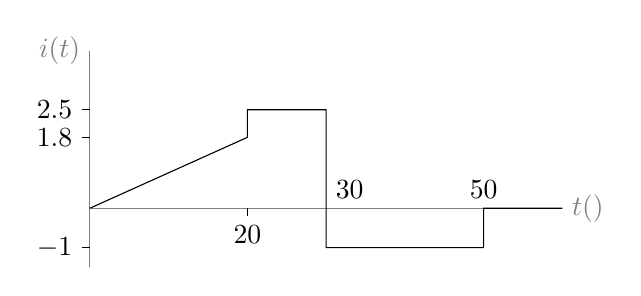
\begin{tikzpicture}
\draw[gray](0,-0.75)--(0,2)node[left]{$i(t)$};
\draw[gray](0,0)--++(6,0)node[right]{$t(\si{\milli\second})$};
\draw(0,0)--++(2,0.9)--++(0,0.35)--++(1,0)--++(0,-1.75)--++(2,0)--++(0,0.5)--++(1,0);
\draw(0,0.9)--++(-0.1,0)node[left]{$\SI{1.8}{\milli\ampere}$};
\draw(0,1.25)--++(-0.1,0)node[left]{$\SI{2.5}{\milli\ampere}$};
\draw(0,-0.5)--++(-0.1,0)node[left]{$\SI{-1}{\milli\ampere}$};
\draw(2,0)--++(0,-0.1)node[below]{$20$};
\draw(3,0)node[above right]{$30$};
\draw(5,0)node[above]{$50$};
\end{tikzpicture}
\caption{(الف)}
\label{شکل_امالہ_مثال_تبدیل_ہوتی_رو_الف}
\end{figure} 

حل:دورانیہ \عددی{t=\SI{0}{\second}} تا \عددی{t=\SI{20}{\milli\second}} میں شرح رو
\begin{align*}
\frac{\dif i}{\dif t}=\frac{\Delta i}{\Delta t}=\frac{\SI{18}{\milli\ampere}-\SI{0}{\milli\ampere}}{\SI{20}{\milli\second}-\SI{0}{\milli\second}}=\SI{0.9}{\ampere\per\second}
\end{align*}
ہے جسے
\begin{align*}
\dif i =0.9 \dif t
\end{align*}
لکھ کر تکمل لیتے ہوئے رو کی مساوات
\begin{align*}
i=\int_{0}^{t} 0.9 \dif t=\left. 0.9  t\right|_{0}^{t}=0.9 t
\end{align*}
حاصل ہوتی ہے۔برق گیر پر ذخیرہ بار دریافت کرنے کی خاطر رو کی مساوات کو 
\begin{align*}
i=\frac{\dif q}{\dif t}=0.9 t
\end{align*}
لکھتے ہوئے تکمل لیتے ہیں۔
\begin{align*}
q=\int_{0}^{t}0.9 t \dif t=\left. 0.45 t^2 \right|_{0}^{t}=0.45 t^2
\end{align*}
مساوات \حوالہ{مساوات_امالہ_بار_دباو_تعلق} سے 
\begin{align*}
v(t)=\frac{q}{C}=\frac{0.45 t^2}{22\times 10^{-6}}=20455 t^2
\end{align*}
لکھا جائے گا اور یوں طاقت کی مساوات
\begin{align*}
p=vi =20455 t^2 \times 0.9 t=18410 t^3
\end{align*}
اور ذخیرہ توانائی کی مساوات
\begin{align*}
w_C=\int_0^t p \dif t=4603 t^4
\end{align*}
ہو گی۔ان مساوات سے لمحہ \عددی{t=\SI{20}{\milli\second}} پر 
\begin{gather}
\begin{aligned}\label{مساوات_امالہ_ابتدائی_قیمتیں_الف}
q(0.02)&=0.45 t^2=0.45\times 0.02^2=\SI{180}{\micro\coulomb}\\
v(0.02)&=20455 t^2=20455\times 0.02^2=\SI{8.182}{\volt}\\
w_C(0.02)&=4603 t^4=4603\times 0.02^4=\SI{737}{\micro\joule}
\end{aligned}
\end{gather}
ہوں گے۔

اسی طرح \عددی{\SI{20}{\milli\second}} تا \عددی{\SI{30}{\milli\second}} دورانیے کے لئے مساوات \حوالہ{مساوات_امالہ_ابتدائی_قیمتیں_الف} میں حاصل کی گئی مقداریں ابتدائی مقداریں تصور کی جائیں گی۔اس دورانیے میں
\begin{align*}
i=\SI{2.5}{\milli\ampere}
\end{align*}
ہے لہٰذا مساوات \حوالہ{مساوات_امالہ_ابتدائی_دباو_الف} کے تحت
\begin{align*}
v&=v(0.02)+\frac{1}{C}\int_{0.02}^t i \dif t\\
&=8.182 +\frac{1}{22\times 10^{-6}}\int_{0.02}^t 2.5\times 10^{-3} \dif t\\
&=33.182+113.636t
\end{align*}
اور
\begin{align*}
p&=iv=0.0025 (33.182+113.636t)=0.083+0.284t\\
w_C&=\frac{C v^2}{2}=\frac{22\times 10^{-6}}{2} (33.182+113.636t)^2
\end{align*}
ہوں گے جن سے اس دورانیے کے آخری لمحے پر
\begin{gather}
\begin{aligned}\label{مساوات_امالہ_ابتدائی_قیمتیں_ب}
v(0.03)&=33.182+113.636\times 0.03=\SI{36.591}{\volt}\\
w_C(0.03)&=\frac{Cv^2}{2}=\frac{22\times 10^{-6} \times 36.591^2}{2}=\SI{14.73}{\milli\joule}
\end{aligned}
\end{gather}
حاصل ہوتے ہیں۔

شکل \حوالہ{شکل_امالہ_مثال_تبدیل_ہوتی_رو_الف} میں \عددی{t=\SI{30}{\milli\second}} تا \عددی{t=\SI{50}{\milli\second}} کے متغیرات حاصل کرتے ہوئے مساوات \حوالہ{مساوات_امالہ_ابتدائی_قیمتیں_ب} کی قیمتیں ابتدائی قیمتیں تصور کی جائیں گی۔پہلے دباو کی مساوات حاصل کرتے ہیں۔
\begin{align*}
v&=v(0.03)+\frac{1}{C}\int_{0.03}^{t}-10^{-3} \dif t\\
&=\left. 36.591-\frac{10^{-3}}{22\times 10^{-6}}t\right|_{0.03}^{t}\\
&=37.955-45.455t
\end{align*}
طاقت کی مساوات درج ذیل ہے
\begin{align*}
p=&iv  \\
&=-0.001(37.955-45.455t)\\
&=-0.038+0.0455t
\end{align*}
جبکہ ذخیرہ توانائی
\begin{align*}
w_C&=\frac{Cv^2}{2}\\
&=\frac{22\times 10^{-6} (37.955-45.455t)^2}{2}
\end{align*}
ہے۔لمحہ \عددی{\SI{50}{\milli\second}} کے بعد رو صفر کے برابر ہے لہٰذا نہ تو برق گیر کا دباو تبدیل ہو گا اور نہ ہی اس میں ذخیرہ توانائی  کی قیمت تبدیل ہو گی۔
\انتہا{مثال}
%=================
\ابتدا{مشق}
شکل \حوالہ{شکل_امالہ_مشق_دباو_سے_رو-الف} میں \عددی{\SI{68}{\micro\farad}} کے برق گیر کا دباو دیا گیا ہے۔رو کی شکل کھینچیں۔

\begin{figure}
\centering
\begin{tikzpicture}
\draw[gray](0,0)--++(0,1.5)node[left]{$v(t)$};
\draw[gray](0,0)--++(6,0)node[right]{$t(\si{\milli\second})$};
\draw(0,0)--(3,1)--(5,0)--(6,0);
\draw(0,1)--++(-0.1,0)node[left]{$\SI{50}{\volt}$};
\draw(3,0)--++(0,-0.1)node[below]{$20$};
\draw(5,0)--++(0,-0.1)node[below]{$30$};
\end{tikzpicture}
\caption{دباو کا خط۔}
\label{شکل_امالہ_مشق_دباو_سے_رو-الف}
\end{figure}

جواب:پہلی \عددی{\SI{20}{\milli\second}} کے لئے \عددی{\SI{0.17}{\ampere}} اور اگلے \عددی{\SI{10}{\milli\second}} کے لئے \عددی{\SI{-0.34}{\ampere}} جبکہ بقایا وقت رو صفر ہے۔
\انتہا{مشق}
%=================
\ابتدا{مشق}
گزشتہ مثال میں لمحہ \عددی{t=\SI{20}{\milli\second}} پر برقی گیر میں ذخیرہ توانائی دریافت کریں۔

جواب:\عددی{\SI{85}{\milli\joule}}
\انتہا{مشق}
%============================
\ابتدا{مشق}
شکل \حوالہ{شکل_امالہ_مشق_دباو_سے_رو-ب} میں \عددی{\SI{2.2}{\micro\farad}} کے برق گیر کا دباو دیا گیا ہے۔رو کی شکل کھینچیں۔لمحہ \عددی{t=\SI{4}{\milli\second}} پر ذخیرہ توانائی دریافت کریں۔لمحہ \عددی{t=\SI{1.5}{\milli\second}} اور \عددی{\SI{5.5}{\milli\second}} پر رو دریافت کریں۔

\begin{figure}
\centering
\begin{tikzpicture}
\draw[gray](0,-1.5)--(0,1.5)node[left]{$v(t)$};
\draw[gray](0,0)--++(7,0)node[right]{$t(\si{\milli\second})$};
\draw(0,0)--(1,1)--(2,1)--(3,-0.5)--(4,-1)--(5,-1)--(6,0)--(7,0);
\foreach \x/\xx in {1/1,2/2,3/3,4/4,5/5,6/6}{\draw (\x,0)--++(0,-0.1)node[below]{$\xx$};}
\foreach \y/\yy in {-1/-10,-0.5/-5,1/10}{\draw(0,\y)--++(-0.1,0)node[left]{$\yy\, \si{\volt}$};}
\end{tikzpicture}
\caption{دباو کا خط۔}
\label{شکل_امالہ_مشق_دباو_سے_رو-ب}
\end{figure}

جواب:\عددی{\SI{110}{\micro\joule}}، \عددی{\SI{0}{\ampere}}، \عددی{\SI{-22}{\milli\ampere}}
\انتہا{مشق}
%=================

\ابتدا{مشق}
شکل \حوالہ{شکل_امالہ_مشق_دباو_سے_رو-پ} میں \عددی{\SI{100}{\micro\farad}} کے برق گیر کی رو دی گئی ہے۔دباو کا خط کھینچیں۔لمحہ \عددی{t=\SI{3}{\milli\second}} پر ذخیرہ توانائی دریافت کریں۔

\begin{figure}
\centering
\begin{tikzpicture}
\draw[gray](0,-2)--(0,1)node[left]{$i(t)$};
\draw[gray](0,0)--++(6,0)node[right]{$t(\si{\milli\second})$};
\draw(0,0)--(2,-1)--(3,-1)--(3,-1.5)--(4,-1.5)--(4,0.5)--(5,0.5)--(5,0)--(6,0);
\foreach \x/\xx in {1/1,2/2,3/3,4/4,5/5}{\draw (\x,0)--++(0,-0.1)node[below]{$\xx$};}
\foreach \y/\yy in {-1.5/-15,-1/-10,0.5/5}{\draw(0,\y)--++(-0.1,0)node[left]{$\yy\, \si{\ampere}$};}
\end{tikzpicture}
\caption{رو کا خط۔}
\label{شکل_امالہ_مشق_دباو_سے_رو-پ}
\end{figure}

جواب:\عددی{\SI{2}{\joule}}
\انتہا{مشق}
%=================

\حصہ{امالہ گیر}
\اصطلاح{امالہ گیر}\فرہنگ{امالہ گیر}\حاشیہب{inductor}\فرہنگ{inductor} عموماً موصل تار کے \اصطلاح{لچھے}\فرہنگ{لچھا}\حاشیہب{coil}\فرہنگ{coil} کی صورت کا ہوتا ہے۔ایسا لچھا کسی \اصطلاح{مقناطیسی مرکز}\فرہنگ{مرکز!مقناطیسی}\فرہنگ{مقناطیسی مرکز}\حاشیہب{magnetic core}\فرہنگ{core!magnetic} یا \اصطلاح{غیر مقناطیسی مرکز}\فرہنگ{غیر مقناطیسی مرکز}\فرہنگ{مرکز!غیر مقناطیسی}\حاشیہب{non-magnetic core}\فرہنگ{core!non-magnetic} پر لپیٹا ہو سکتا ہے۔ مقناطیسی مرکز کے لچھے \اصطلاح{ٹرانسفارمر}\فرہنگ{ٹرانسفارمر}\حاشیہب{transformer}\فرہنگ{transformer} اور \اصطلاح{فلٹر}\فرہنگ{فلٹر}\حاشیہب{filter}\فرہنگ{filter} میں استعمال کئے جاتے ہیں جبکہ غیر مقناطیسی مرکز کے لچھے مواصلاتی نظام میں اہم کردار ادا کرتے ہیں۔

تاریخی طور پر پہلے یہ معلوم ہوا کہ رو گزارتی تار کے گرد مقناطیسی میدان پیدا ہوتا ہے۔ایسی مقناطیسی میدان اور میدان پیدا کرنے والی رو کے مابین راست تناسبی تعلق پایا جاتا ہے۔اس کے بعد معلوم ہوا کہ بدلتا مقناطیسی میدان برقی دباو پیدا کرتا ہے جہاں دباو اور مقناطیسی میدان پیدا کرنے والی رو کی شرح کے مابین راست تناسبی تعلق پایا جاتا ہے۔اسی تعلق کو درج ذیل مساوات پیش کرتی ہے
\begin{align}\label{مساوات_امالہ_بنیادی_مساوات_امالہ_الف}
v=L \frac{\dif i}{\dif t}
\end{align}
جہاں تناسبی مستقل کو \عددی{L} لکھا اور \اصطلاح{امالہ}\فرہنگ{امالہ}\حاشیہب{inductance}\فرہنگ{inductance} پکارا جاتا ہے۔امالہ کی اکائی\حاشیہد{امالہ کی اکائی امریکی تخلیق کار یوسف ہینری کے نام سے منسوب ہے۔} کو \اصطلاح{ہینری}\فرہنگ{ہینری}\حاشیہب{Henry}\فرہنگ{Henry} پکارا اور \عددی{\si{\henry}} سے ظاہر کیا جاتا ہے۔آپ دیکھ سکتے ہیں کہ ایک وولٹ سیکنڈ فی ایمپیئر \عددی{\si{\volt\second\per\ampere}} کو ہینری کہا گیا ہے۔ 

اس مساوات کی تکمل صورت سے رو حاصل ہوتی ہے
\begin{align}
i=\int_{-\infty}^{t}\frac{1}{L} v \dif t
\end{align}
جہاں ازل \عددی{-\infty} سے لمحہ \عددی{t} تک تکمل لیا گیا ہے۔مستقل قیمت کی امالہ کی صورت میں \عددی{L} کو تکمل کے باہر نکالا جا سکتا ہے۔
\begin{align}
i=\frac{1}{L}\int_{-\infty}^{t} v \dif t
\end{align}
اس تکمل کو دو ٹکڑوں میں لکھا جا سکتا ہے 
\begin{gather}
\begin{aligned}
i&=\frac{1}{L}\int_{-\infty}^{t_0} v \dif t+\frac{1}{L} \int_{t_0}^{t} v \dif t\\
&=i(t_0)+\frac{1}{L} \int_{t_0}^{t} v \dif t
\end{aligned}
\end{gather}
جہاں پہلا ٹکڑا ازل سے \عددی{t_0} تک اور دوسرا ٹکڑا \عددی{t_0} سے \عددی{t} حاصل کیا گیا ہے۔مندرجہ بالا مساوات میں لمحہ \عددی{t_0} پر امالہ گیر کی رو کو \عددی{i(t_0)} کہا گیا ہے۔

امالہ کو فراہم طاقت سے امالہ کو منتقل توانائی \عددی{w_L} دریافت کی جا سکتی ہے۔
\begin{align}
p=vi
\end{align}
سے
\begin{align}\label{مساوات_امالہ_کو_مہیا_طاقت_الف}
p=\frac{\dif w_L}{\dif t}=\left[L \frac{\dif i}{\dif t}\right] i
\end{align}
لکھتے ہوئے اور تکمل لینے سے
\begin{align*}
w_L&=\int_{-\infty}^{t} \left[L\frac{\dif i}{\dif t}\right]i\dif t\\
&=L\int_{0}^{i} i \dif i
\end{align*}

\begin{align}
w_L=\frac{Li^2}{2}
\end{align}
حاصل ہوتا ہے جہاں وقت کی ابتدا \عددی{t=-\infty} پر \عددی{i=0} تصور کی گئی ہے۔

تصور کریں کہ ایک دور میں یک سمتی رو پائی جاتی ہو۔اب یک سمتی رو وقت کے ساتھ تبدیل نہیں ہوتی لہٰذا مساوات \حوالہ{مساوات_امالہ_بنیادی_مساوات_امالہ_الف} کے تحت اس دور میں موجود امالہ پر دباو صفر کے برابر ہو گا۔ہم کہہ سکتے ہیں کہ یک سمتی رو کی نقطہ نظر سے امالہ بطور قصر دور کردار ادا کرتی ہے۔یوں کسی بھی دور کا یک سمتی تجزیہ کرتے ہوئے دور میں موجود تمام امالہ کو قصر دور تصور کیا جاتا ہے۔

امالہ میں فوراً رو تبدیل کرنے کے لئے مساوات \حوالہ{مساوات_امالہ_کو_مہیا_طاقت_الف} کے تحت  لامحدود طاقت درکار ہو گی۔کائنات میں لامحدود طاقت کا منبع کہیں نہیں پایا جاتا لہٰذا امالہ کی رو کو فوراً تبدیل کرنا ناممکن ہے۔اس حقیقت کی مساواتی صورت درج ذیل ہے۔
\begin{align}\label{مساوات_امالہ_امالہ_گیر_رو_بلا_جوڑ_ہے}
i_L(t_+)=i_L(t_-)
\end{align}
مساوات \حوالہ{مساوات_امالہ_امالہ_گیر_رو_بلا_جوڑ_ہے} کے تحت امالہ گیر کی رو کسی بھی لمحے \عددی{t} کے فوراً بعد \عددی{t_+} اور اس لمحے کے فوراً  پہلے \عددی{t_-} برابر ہوں گے۔یوں امالہ گیر کی رو \اصطلاح{بلا جوڑ تفاعل}\فرہنگ{بلا جوڑ!تفاعل}\فرہنگ{تفاعل!بلا جوڑ}\حاشیہب{continuous function}\فرہنگ{function!continuous}\فرہنگ{continuous!function} ہے جس میں \اصطلاح{سیڑھی نما}\فرہنگ{سیڑھی نما}\فرہنگ{step} یکدم تبدیلی ممکن نہیں ہے۔یہ ایک اہم نتیجہ ہے جس کے تحت دور میں سوئچ کو چالو سے غیر چالو (یا غیر چالو سے چالو) کرنے کے فوراً بعد امالہ میں رو کی قیمت وہی ہو گی جو سوئچ چالو (یا غیر چالو) کرنے سے پہلے تھی۔

%=============================
\ابتدا{مثال}\شناخت{مثال_امالہ_یکسمتی_دور_الف}
شکل \حوالہ{شکل_امالہ_یکسمتی_دور_الف} میں ذخیرہ توانائی دریافت کریں۔

\begin{figure}
\centering
\begin{subfigure}{1\textwidth}
\centering
\begin{tikzpicture}
\draw(0,0) to [american voltage source,l={$\SI{10}{\volt}$}]++(0,\y) to [inductor,l={${L_1=\SI{2}{\milli\henry}}$}]++(\x,0) to [resistor,l={$\SI{6}{\ohm}$}]++(\x,0) to [inductor,l={${L_2=\SI{1}{\milli\henry}}$}]++(\x,0) to [resistor,l={$\SI{5}{\ohm}$}]++(\x,0) to [short]++(\x,0) to [resistor,l={$\SI{2}{\ohm}$}]++(0,-\y) to [short] (0,0);
\draw(\x,0) to [capacitor,*-*,l={$\SI{3}{\micro\farad}$}]++(0,\y);
\draw(3*\x,0) to [american current source,*-*,l={$\SI{4}{\ampere}$}]++(0,\y);
\draw(4*\x,0) to [capacitor,*-*,l={$\SI{10}{\micro\farad}$}]++(0,\y);
\draw(\x-\dx,1/4*\y)node[left]{$C_1$};
\draw(4*\x-\dx,1/4*\y)node[left]{$C_2$};
\end{tikzpicture}
\caption*{(الف)}
\end{subfigure}
\begin{subfigure}{1\textwidth}
\centering
\begin{tikzpicture}
\draw(0,0) to [american voltage source,l={$\SI{10}{\volt}$}]++(0,\y) to [short]++(\x,0) to [resistor,l={$\SI{6}{\ohm}$}]++(\x,0) to [short,i={$I_1$}]++(\x,0) to [resistor,l={$\SI{5}{\ohm}$}]++(\x,0) to [short,i={$I_2$}]++(\x,0) to [resistor,l={$\SI{2}{\ohm}$}]++(0,-\y) to [short] (0,0);
\draw(3*\x,0)node[ground]{} to [american current source,*-*,l={$\SI{4}{\ampere}$}]++(0,\y)node[above]{$J$};
\draw(\x,0) to [short,*-o]++(0,\y/8);
\draw(\x,\y) to [short,*-o]++(0,-\y/8);
\draw(4*\x,0) to [short,*-o]++(0,\y/8);
\draw(4*\x,\y) to [short,*-o]++(0,-\y/8);
\draw(\x+\dx/2,\y/2)node{$\begin{aligned}&+ \\& V_{C1} \\ &- \end{aligned}$};
\draw(4*\x+\dx/2,\y/2)node{$\begin{aligned}&+ \\& V_{C2} \\ &- \end{aligned}$};
\end{tikzpicture}
\caption*{(ب)}
\end{subfigure}
\caption{مثال \حوالہ{مثال_امالہ_یکسمتی_دور_الف} کا دور۔}
\label{شکل_امالہ_یکسمتی_دور_الف}
\end{figure}

حل:اس دور میں صرف یک سمتی منبع پائے جاتے ہیں۔ہم اس حقیقت پر بحث کر چکے ہیں کہ یک سمتی ادوار میں امالہ کو قصر دور اور برق گیر کو کھلا دور تصور کیا جاتا ہے۔ایسا ہی کرتے ہوئے  شکل-ب حاصل ہوتا ہے جسے آپ اپنی پسندیدہ  ترکیب سے حل کر سکتے ہیں۔نچلی جوڑ کو زمین لیتے ہوئے جوڑ \عددی{J} پر کرخوف مساوات رو
\begin{align*}
I_1+4=I_2
\end{align*} 
جبکہ بیرونی دائرے پر کرخوف مساوات دباو
\begin{align*}
10=6I_1+(5+2)I_2
\end{align*}
 لکھتے ہیں۔انہیں حل کرتے ہوئے درج ذیل حاصل ہوتا ہے۔
\begin{align*}
I_1&=-\frac{18}{13}\, \si{\ampere}\\
I_2&=\frac{34}{13}\,\si{\ampere}
\end{align*}
برق گیر \عددی{C_1} پر دباو شکل کو دیکھ کر لکھی جا سکتی ہے  جبکہ \عددی{C_2}  پر دباو کو اوہم کے قانون کی مدد سے لکھا جا سکتا ہے۔
\begin{align*}
V_{C1}&=\SI{10}{\volt}\\
V_{C2}&=2 \times \frac{34}{13}=\frac{68}{13}\,\volt
\end{align*}
ان حقائق کو استعمال کرتے ہوئے برق گیر اور امالہ میں ذخیرہ توانائی دریافت کر سکتے ہیں۔
\begin{align*}
w_{C1}&=\frac{3\times 10^{-6} \times 10^2}{2}=\SI{0.15}{\milli\joule}\\
w_{C2}&=\frac{10 \times 10^{-6} \left(\frac{68}{13}\right)^2}{2}=\SI{0.14}{\milli\joule}\\
w_{L1}&=\frac{0.002\times \left(\frac{18}{13}\right)^2 }{2}=\SI{1.92}{\milli\joule}\\
w_{L2}&=\frac{0.001\times \left(\frac{18}{13}\right)^2}{2}=\SI{0.96}{\milli\joule}
\end{align*}
\انتہا{مثال}
%================================
\ابتدا{مثال}\شناخت{مثال_امالہ_یکسمتی_دور_ب}
امالہ کی رو کے خط کو شکل \حوالہ{شکل_امالہ_یکسمتی_دور_ب}-الف میں دکھایا گیا ہے۔اس کے دباو کا خط کھینچیں۔امالہ کی قیمت \عددی{\SI{30}{\milli\henry}} ہے۔

\begin{figure}
\centering
\begin{subfigure}{0.5\textwidth}
\begin{tikzpicture}
\draw[gray](0,0)--++(4,0)node[right]{$t(\si{\milli\second})$};
\draw[gray](0,-2.5)--(0,1.5)node[left]{$i(t)$};
\draw(-0.5,0)--(0,0)--(2,1)--(3,0)--(4,0);
\draw(0,1)--++(-0.1,0)node[left]{$\SI{60}{\milli\ampere}$};
\draw(2,0)--++(0,-0.1)node[below]{$20$};
\draw(3,0)--++(0,-0.1)node[below]{$30$};
\end{tikzpicture}
\caption*{(الف)}
\end{subfigure}%
\begin{subfigure}{0.5\textwidth}
\begin{tikzpicture}
\draw[gray](0,0)--++(4,0)node[right]{$t(\si{\milli\second})$};
\draw[gray](0,-2.5)--(0,1.5)node[left]{$i(t)$};
\draw(-0.5,0)--(0,0)--(0,1)--(2,1)--(2,-2)--(3,-2)--(3,0)--(4,0);
\draw(0,1)node[left]{$\SI{90}{\milli\volt}$};
\draw(0,-2)node[left]{$\SI{180}{\milli\volt}$};
\draw(2,0)--++(0,-0.1)node[below left]{$20$};
\draw(3,0)--++(0,-0.1)node[below right]{$30$};
\end{tikzpicture}
\caption*{(ب)}
\end{subfigure}%
\caption{مثال \حوالہ{مثال_امالہ_یکسمتی_دور_ب} کا دور۔}
\label{شکل_امالہ_یکسمتی_دور_ب}
\end{figure}

حل:امالہ گیر کی رو سے امالہ گیر کا دباو مساوات \حوالہ{مساوات_امالہ_بنیادی_مساوات_امالہ_الف} کی مدد سے حاصل کیا جاتا ہے۔وقت \عددی{t=-\infty} تا \عددی{t=0} رو صفر کے برابر ہے لہٰذا
\begin{align*}
v=30\times 10^{-3} \left(\frac{0}{-\infty-0}\right)=\SI{0}{\volt}
\end{align*}
ہو گا۔اگلا دورانیہ \عددی{t=0} تا \عددی{t=\SI{20}{\milli\second}} ہے جس میں رو کی قیمت  یکساں شرح سے مسلسل بڑھتے ہوئے \عددی{i=0} سے \عددی{i=\SI{60}{\milli\ampere}} ہو جاتی ہے لہٰذا اس دوران
\begin{align*}
v=30\times 10^{-3} \left(\frac{0.06-0}{0.02-0}\right)=\SI{90}{\milli\volt}
\end{align*}
ہو گا۔دورانیہ \عددی{\SI{20}{\milli\second}} تا \عددی{\SI{30}{\milli\second}} میں دباو درج ذیل ہو گا۔
\begin{align*}
v=30\times 10^{-3} \left(\frac{0-0.06}{0.03-0.02}\right)=\SI{-180}{\milli\volt}
\end{align*}
\عددی{\SI{30}{\milli\second}} کے بعد رو صفر رہتی ہے لہٰذا
\begin{align*}
v=30\times 10^{-3} \left(\frac{0}{\infty-0.03}\right)=\SI{0}{\volt}
\end{align*}
ہو گا۔ان نتائج کو شکل \حوالہ{شکل_امالہ_یکسمتی_دور_ب}-ب میں دکھایا گیا ہے۔
\انتہا{مثال}
%================================
\ابتدا{مثال}
امالہ گیر کی رو \عددی{i(t)=5\cos 377 t} جبکہ اس کی امالہ \عددی{\SI{100}{\milli\henry}} ہے۔امالہ گیر کا دباو اور اس میں ذخیرہ توانائی کی مساوات حاصل کریں۔

حل: مساوات \حوالہ{مساوات_امالہ_بنیادی_مساوات_امالہ_الف}  سے دباو درج ذیل لکھا جاتا ہے۔
\begin{align*}
v&=L \frac{\dif i}{\dif t}\\
&=0.1 \times (-5 \times 377 \sin 377 t)\\
&=-188.5 \sin 377 t \quad \si{\volt}
\end{align*}
ذخیرہ توانائی کو درج ذیل لکھا جا سکتا ہے۔
\begin{align*}
w_L(t)&=\frac{L i^2}{2}\\
&=\frac{0.1 \times \left(5\cos 377 t\right)^2}{2}\\
&=1.25 \cos^2 377t \, \si{\joule}
\end{align*}
\انتہا{مثال}
%==================================
\ابتدا{مشق}\شناخت{مشق_امالہ_رو_دباو_خط_الف}
رو کا خط شکل \حوالہ{شکل_امالہ_مشق_رو_دباو_خط_الف} میں دکھایا گیا ہے۔دباو کا خط کھینچیں۔امالہ کی قیمت \عددی{\SI{2}{\henry}} ہے۔

\begin{figure}
\centering
\begin{subfigure}{0.5\textwidth}
\centering
\begin{tikzpicture}
\draw[gray](0,-1.35)--(0,1.5)node[left]{$i(t)$};
\draw[gray](0,0)--++(4.25,0)node[right]{$t(\si{\milli\second})$};
\draw(-0.25,0)--(0,0)--(2,1)--(3,1)--(4,0)--(4.25,0);
\draw(0,1)node[left]{$\SI{12}{\ampere}$};
\draw(2,0)node[below]{$2$};
\draw(3,0)node[below]{$3$};
\draw(4,0)node[below]{$4$};
\end{tikzpicture}
\caption*{(الف)}
\end{subfigure}%
\begin{subfigure}{0.5\textwidth}
\centering
\begin{tikzpicture}
\draw[gray](0,-1.35)--(0,1.5)node[left]{$v(t)$};
\draw[gray](0,0)--++(4.25,0)node[right]{$t(\si{\milli\second})$};
\draw(-0.25,0) --(0,0)--(0,0.6)--(2,0.6)--(2,0)--(3,0)--(3,-1.2)--(4,-1.2)--(4,0)--(4.25,0);
\draw(0,0.6)node[left]{$\SI{12}{\volt}$};
\draw(0,-1.2)node[left]{$\SI{-24}{\volt}$};
\draw(2,0)node[below]{$2$};
\draw(3,0)node[above]{$3$};
\draw(4,0)node[above]{$4$};
\end{tikzpicture}
\caption*{(ب)}
\end{subfigure}%
\caption{مشق \حوالہ{مشق_امالہ_رو_دباو_خط_الف} کا دور۔}
\label{شکل_امالہ_مشق_رو_دباو_خط_الف}
\end{figure}

جواب:شکل \حوالہ{شکل_امالہ_مشق_رو_دباو_خط_الف}-ب میں دباو کا خط دکھایا گیا ہے۔
\انتہا{مشق}
%=================================
\ابتدا{مشق}
گزشتہ مشق میں لمحہ \عددی{t=\SI{3.5}{\milli\second}} پر امالہ گیر میں ذخیرہ توانائی دریافت کریں۔

جواب:\عددی{\SI{36}{\joule}}
\انتہا{مشق}
%===========================
\ابتدا{مشق}\شناخت{مشق_امالہ_رو_دباو_خط_ب}
پانچ ہینری امالہ گیر کا دباو شکل \حوالہ{شکل_امالہ_مشق_رو_دباو_خط_ب}-الف میں دکھایا گیا ہے۔رو کا خط کھینچیں۔

\begin{figure}
\centering
\begin{subfigure}{0.5\textwidth}
\centering
\begin{tikzpicture}
\draw[gray](0,0)--(4.25,0)node[right]{$t(\si{\milli\second})$};
\draw[gray](0,-1)--(0,2.5)node[left]{$v(t)$};
\draw(-0.25,0)--(0,0)--(0,2)--(2,2)--(2,1)--(3,1)--(3,-0.5)--(4,-0.5)--(4,0)--(4.25,0);
\draw(0,-0.5)node[left]{$\SI{-50}{\volt}$};
\draw(0,1)node[left]{$\SI{100}{\volt}$};
\draw(0,2)node[left]{$\SI{200}{\volt}$};
\draw(1,0)--++(0,-0.1)node[below]{$1$};
\draw(2,0)--++(0,-0.1)node[below]{$2$};
\draw(3,0)++(0,-0.1)node[below left]{$3$};
\draw(4,0)node[above]{$4$};
\end{tikzpicture}
\caption*{(الف)}
\end{subfigure}%
\begin{subfigure}{0.5\textwidth}
\centering
\begin{tikzpicture}
\draw[gray](0,0)--(4.25,0)node[right]{$t(\si{\milli\second})$};
\draw[gray](0,-1)--(0,2.5)node[left]{$i(t)$};
\draw(-0.25,0)--(0,0)--(2,1.6)--(3,2)--(4,1.8)--(4.25,1.8);
\draw(0,1.6)--++(-0.1,0)node[below left]{$\SI{80}{\ampere}$};
\draw(0,1.8)--++(-0.1,0)node[left]{$\SI{90}{\ampere}$};
\draw(0,2)--++(-0.1,0)node[above left]{$\SI{100}{\ampere}$};
\draw(1,0)--++(0,-0.1)node[below]{$1$};
\draw(2,0)--++(0,-0.1)node[below]{$2$};
\draw(3,0)--++(0,-0.1)node[below]{$3$};
\draw(4,0)--++(0,-0.1)node[below]{$4$};
\end{tikzpicture}
\caption*{(ب)}
\end{subfigure}%
\caption{مشق \حوالہ{مشق_امالہ_رو_دباو_خط_ب} کا دور۔}
\label{شکل_امالہ_مشق_رو_دباو_خط_ب}
\end{figure}

جواب:رو کا خط شکل \حوالہ{شکل_امالہ_مشق_رو_دباو_خط_ب}-ب میں دکھایا گیا ہے۔
\انتہا{مشق}
%=============================
\ابتدا{مشق}\شناخت{مشق_امالہ_رو_دباو_خط_پ}
امالہ گیر کے دباو کا خط شکل \حوالہ{شکل_امالہ_مشق_رو_دباو_خط_پ} میں دکھایا گیا ہے۔لمحہ \عددی{t=0} پر \عددی{i(0)=\SI{0.1}{\ampere}} کی صورت میں رو کا خط حاصل کریں۔امالہ \عددی{\SI{0.1}{\henry}} کے برابر ہے۔ لمحہ \عددی{t=\SI{3}{\milli\second}} پر امالہ گیر میں ذخیرہ توانائی دریافت کریں۔

\begin{figure}
\centering
\begin{subfigure}{0.5\textwidth}
\centering
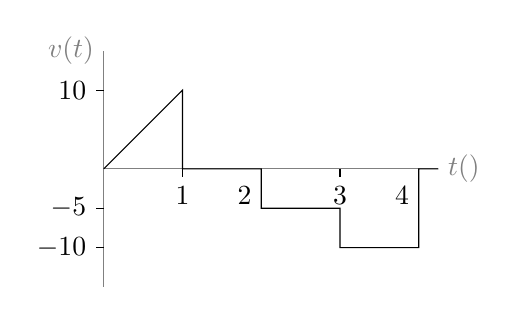
\begin{tikzpicture}
\draw[gray](0,0)--(4.25,0)node[right]{$t(\si{\milli\second})$};
\draw[gray](0,-1.5)--(0,1.5)node[left]{$v(t)$};
\draw(0,0)--(1,1)--(1,0)--(2,0)--(2,-0.5)--(3,-0.5)--(3,-1)--(4,-1)--(4,0)--(4.25,0);
\draw(0,1)--++(-0.1,0)node[left]{$\SI{10}{\volt}$};
\draw(0,-1)--++(-0.1,0)node[left]{$\SI{-10}{\volt}$};
\draw(0,-0.5)--++(-0.1,0)node[left]{$\SI{-5}{\volt}$};
\draw(1,0)--++(0,-0.1)node[below]{$1$};
\draw(2,0)--++(0,-0.1)node[below left]{$2$};
\draw(3,0)--++(0,-0.1)node[below]{$3$};
\draw(4,0)--++(0,-0.1)node[below left]{$4$};
\end{tikzpicture}
\caption*{(الف)}
\end{subfigure}%
\begin{subfigure}{0.5\textwidth}
\centering
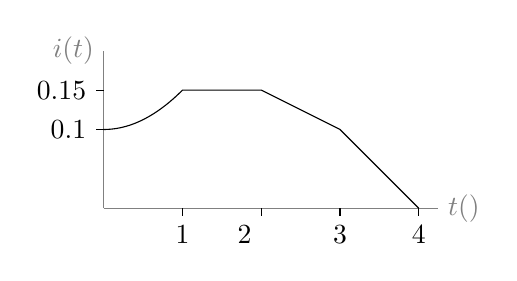
\begin{tikzpicture}
\draw[gray](0,0)--(4.25,0)node[right]{$t(\si{\milli\second})$};
\draw[gray](0,0)--(0,2)node[left]{$i(t)$};
\draw(0,1)
\foreach \kx in {0,0.01,...,1}{--(\kx,1+0.5*\kx*\kx)}--(1,1.5)--(2,1.5)--(3,1)--(4,0);
\draw(0,1)--++(-0.1,0)node[left]{$\SI{0.1}{\ampere}$};
\draw(0,1.5)--++(-0.1,0)node[left]{$\SI{0.15}{\ampere}$};
%\draw(0,-0.5)--++(-0.1,0)node[left]{$\SI{-5}{\volt}$};
\draw(1,0)--++(0,-0.1)node[below]{$1$};
\draw(2,0)--++(0,-0.1)node[below left]{$2$};
\draw(3,0)--++(0,-0.1)node[below]{$3$};
\draw(4,0)--++(0,-0.1)node[below]{$4$};
\end{tikzpicture}
\caption*{(ب)}
\end{subfigure}%
\caption{مشق \حوالہ{مشق_امالہ_رو_دباو_خط_پ} کا دور۔}
\label{شکل_امالہ_مشق_رو_دباو_خط_پ}
\end{figure}

جواب:رو کا خط شکل \حوالہ{شکل_امالہ_مشق_رو_دباو_خط_پ} میں دکھایا گیا ہے۔لمحہ \عددی{t=\SI{3}{\milli\second}} پر \عددی{w_L(\SI{3}{\milli\second})=\SI{0.5}{\milli\joule}} ہے۔
\انتہا{مشق}
%=============================
\ابتدا{مشق}\شناخت{مشق_امالہ_رو_دباو_خط_ت}
شکل \حوالہ{شکل_امالہ_مشق_رو_دباو_خط_ت} میں \عددی{\SI{1}{\milli\henry}}، \عددی{\SI{4}{\milli\henry}}، \عددی{\SI{3}{\micro\farad}} اور \عددیء{\SI{4}{\micro\farad}} میں ذخیرہ توانائی دریافت کریں۔

\begin{figure}
\centering
\begin{tikzpicture}
\draw(0,0) to [american voltage source,l={$\SI{10}{\volt}$}]++(0,\y) to [resistor,l={$\SI{2}{\ohm}$}]++(0,\y) to [short]++(\x,0) to [inductor,l={$\SI{1}{\milli\henry}$}]++(\x,0) to [resistor,l={$\SI{6}{\ohm}$}]++(\x,0) to [inductor,l={$\SI{4}{\milli\henry}$}]++(\x,0) to [resistor,l={$\SI{10}{\ohm}$}]++(0,-2*\y) to [short] (0,0);
\draw(\x,2*\y) to [short,*-]++(0,\y) to [american current source,l={$\SI{2}{\ampere}$}]++(3*\x,0) to [short,-*]++(0,-\y);
\draw(\x,0) to [capacitor,*-*,l={$\SI{3}{\micro\farad}$}]++(0,2*\y);
\draw(2*\x,0) to [resistor,*-,l={$\SI{8}{\ohm}$}]++(0,\y) to [capacitor,-*,l={$\SI{4}{\micro\farad}$}]++(0,\y);
\end{tikzpicture}
\caption{مشق \حوالہ{مشق_امالہ_رو_دباو_خط_ت} کا دور۔}
\label{شکل_امالہ_مشق_رو_دباو_خط_ت}
\end{figure}

جوابات:\عددی{\SI{302}{\micro\joule}}، \عددی{\SI{0.907}{\micro\joule}}، \عددی{\SI{85.6}{\micro\joule}}، \عددی{\SI{114}{\micro\joule}}
\انتہا{مشق}
%=============================

\حصہ{برق گیر اور امالہ گیر کے خصوصیات}
برقی گنجائش، برقی گنجائش  کی قیمت میں خلل اور دباو، برق گیر کے  اہم خصوصیات ہیں۔ معیاری برق گیر چند \عددی{\si{\pico\farad}} سے تقریباً \عددی{\SI{50}{\milli\farad}} تک کی قیمتوں میں عام دستیاب ہے۔ان سے کم اور زیادہ قیمتیں بھی دستیاب ہیں۔ یہ برق گیر عموماً \عددی{\SI{6.3}{\volt}} تا \عددی{\SI{500}{\volt}} تک کے مختلف دباو کے لئے دستیاب ہیں۔زیادہ دباو کے برق گیر بھی دستیاب ہیں۔برق گیر کو اس کی معین دباو سے زیادہ دباو پر ہرگز استعمال نہ کریں چونکہ ایسا کرنے سے  برق گیر تباہ ہو سکتا ہے۔برقی گنجائش میں خلل کی عمومی قیمتیں \عددی{\SI{\mp 5}{\percent}}، \عددی{\SI{\mp 10}{\percent}} اور \عددی{\SI{\mp 20}{\percent}} ہیں۔ جدول \حوالہ{جدول_امالہ_معیاری_برقی_گنجائش} میں معیاری دستیاب برقی گیر کی گنجائش دی گئی ہے۔
%==============================

\begin{table}\caption{معیاری برق گیر کے گنجائش کی قیمتیں۔}
\centering
\begin{tabular}{lllllllllll}
$\si{\pico\farad}$ & $\si{\pico\farad}$ & $\si{\pico\farad}$ & $\si{\pico\farad}$ & $\si{\micro\farad}$ & $\si{\micro\farad}$ &  $\si{\micro\farad}$ &  $\si{\micro\farad}$ &  $\si{\micro\farad}$ &  $\si{\micro\farad}$ &  $\si{\micro\farad}$ \\
\hline
$1$ & $10$ &$100$ & $1000$ &$0.010$ & $0.10$ &$1.0$ & $10$ &$100$ & $1000$ & $\num{10000}$\\
 & $12$ &$120$ & $1200$ &$0.012$ & $0.12$ &$1.2$ & $12$ &$120$ & $1200$ & $\num{12000}$\\
 $1.5$& $15$ &$150$ & $1500$ &$0.015$ & $0.15$ &$1.5$ & $15$ &$150$ & $1500$ & $\num{15000}$\\
 & $18$ &$180$ & $1800$ &$0.018$ & $0.18$ &$1.8$ & $18$ &$180$ & $1800$ & $\num{18000}$\\
$2$ & $20$ &$200$ & $2000$ &$0.020$ & $0.20$ &$2.0$ & $20$ &$200$ & $2000$ & $\num{20000}$\\
 & $22$ &$220$ & $2200$ &$0.022$ & $0.22$ &$2.2$ & $22$ &$220$ & $2200$ & $\num{22000}$\\
 & $27$ &$270$ & $2700$ &$0.027$ & $0.27$ &$2.7$ & $27$ &$270$ & $2700$ & $\num{27000}$\\
$3$ & $33$ &$330$ & $3300$ &$0.330$ & $0.33$ &$3.3$ & $33$ &$330$ & $3300$ & $\num{33000}$\\
$4$ & $39$ &$390$ & $3900$ &$0.390$ & $0.39$ &$3.9$ & $39$ &$390$ & $3900$ & $\num{39000}$\\
$5$ & $47$ &$470$ & $4700$ &$0.470$ & $0.47$ &$3.3$ & $47$ &$470$ & $4700$ & $\num{47000}$\\
$6$ & $51$ &$510$ & $5100$ &$0.510$ & $0.51$ &$3.3$ & $51$ &$510$ & $5100$ & $\num{51000}$\\
$7$ & $56$ &$560$ & $5600$ &$0.560$ & $0.56$ &$3.3$ & $56$ &$560$ & $5600$ & $\num{56000}$\\
$8$ & $68$ &$680$ & $6800$ &$0.680$ & $0.68$ &$3.3$ & $68$ &$680$ & $6800$ & $\num{68000}$\\
$9$ & $82$ &$820$ & $8200$ &$0.820$ & $0.82$ &$3.3$ & $82$ &$820$ & $8200$ & $\num{82000}$
\end{tabular}
\label{جدول_امالہ_معیاری_برقی_گنجائش}
\end{table}
%==============================

امالہ گیر کو موصل تار سے بنایا جاتا ہے لہٰذا نہ چاہتے ہوئے بھی اس کی مزاحمت ہو گی۔ امالہ گیر کے اہم خصوصیات اس کی امالہ اور مزاحمت ہیں۔امالہ گیر \عددی{\SI{1}{\nano\henry}} تا \عددی{\SI{100}{\milli\henry}} کی قیمتوں میں عام دستیاب ہے۔اس سے کم یا زیادہ قیمتیں بھی دستیاب ہیں۔امالہ کی قیمتیں \عددی{\SI{\mp 5}{\percent}} اور \عددی{\SI{\mp 10}{\percent}} کے خلل میں دستیاب ہیں۔جدول \حوالہ{جدول_امالہ_امالہ_عمومی_دستیاب_قیمتیں} میں امالہ کی عمومی دستیاب قیمتیں دی گئی ہیں۔

\begin{table}\caption{امالہ کی عمومی دستیاب قیمتیں۔}
\centering
\begin{tabular}{lllllllll}
$\si{\nano\henry}$ & $\si{\nano\henry}$ &$\si{\nano\henry}$ &$\si{\micro\henry}$ &$\si{\micro\henry}$ &$\si{\micro\henry}$ &$\si{\milli\henry}$ &$\si{\milli\henry}$ &$\si{\milli\henry}$ \\
\hline
$1$ & $10$ &$100$ & $1.0$ & $10$ &$100$ & $1.0$ & $10$ & $100$ \\
$1.2$ & $12$ &$120$ & $1.2$ & $12$ &$120$ & $1.2$ & $12$ &  \\
$1.5$ & $15$ &$150$ & $1.5$ & $15$ &$150$ & $1.5$ & $15$ &  \\
$1.8$ & $18$ &$180$ & $1.8$ & $18$ &$180$ & $1.8$ & $18$ &  \\
$2$ & $20$ &$200$ & $2.0$ & $20$ &$200$ & $2.0$ & $20$ &  \\
$2.2$ & $22$ &$220$ & $2.2$ & $22$ &$220$ & $2.2$ & $22$ &  \\
$2.7$ & $27$ &$270$ & $2.7$ & $27$ &$270$ & $2.7$ & $27$ &  \\
$3$ & $33$ &$330$ & $3.3$ & $33$ &$330$ & $3.3$ & $33$ &  \\
$4$ & $39$ &$390$ & $3.9$ & $39$ &$390$ & $3.9$ & $39$ &  \\
$5$ & $47$ &$470$ & $4.7$ & $47$ &$470$ & $4.7$ & $47$ &  \\
$6$ & $51$ &$510$ & $5.1$ & $51$ &$510$ & $5.1$ & $51$ &  \\
$7$ & $56$ &$560$ & $5.6$ & $56$ &$560$ & $5.6$ & $56$ &  \\
$8$ & $68$ &$680$ & $6.8$ & $68$ &$680$ & $6.8$ & $68$ &  \\
$9$ & $82$ &$820$ & $8.2$ & $82$ &$820$ & $8.2$ & $82$ &  
\end{tabular}
\label{جدول_امالہ_امالہ_عمومی_دستیاب_قیمتیں}
\end{table}

%===================
\ابتدا{مثال}\شناخت{مثال_امالہ_گنجائش_اور_قیمتیں_الف}
شکل \حوالہ{شکل_امالہ_گنجائش_اور_قیمتیں_الف}-الف میں \عددی{\SI{100}{\nano\farad}} برق گیر کا دباو دکھایا گیا ہے۔برقی گنجائش میں خلل \عددی{\SI{\mp 10}{\percent}} ممکن ہے۔کم سے کم اور زیادہ سے زیادہ گنجائش کی صورت میں رو کے خط حاصل کریں۔اس برقی گنجائش کو عموماً \عددی{\SI{100}{\nano\farad}\SI{\mp10}{\percent}} لکھا جاتا ہے۔

\begin{figure}
\centering
\begin{subfigure}{0.5\textwidth}
\centering
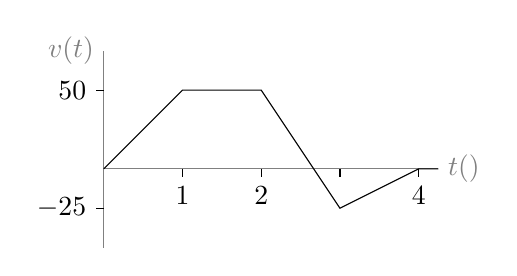
\begin{tikzpicture}
\draw[gray](0,-1)--(0,1.5)node[left]{$v(t)$};
\draw[gray](0,0)--(4.25,0)node[right]{$t(\si{\micro\second})$};
\draw(0,0)--(1,1)--(2,1)--(3,-0.5)--(4,0)--(4.25,0);
\draw(0,1)--++(-0.1,0)node[left]{$\SI{50}{\volt}$};
\draw(0,-0.5)--++(-0.1,0)node[left]{$\SI{-25}{\volt}$};
\draw(1,0)--++(0,-0.1)node[below]{$1$};
\draw(2,0)--++(0,-0.1)node[below]{$2$};
\draw(3,0)--++(0,-0.1);
\draw(4,0)--++(0,-0.1)node[below]{$4$};
\end{tikzpicture}
\caption*{(الف) برق گیر کا دباو۔}
\end{subfigure}%
\begin{subfigure}{0.5\textwidth}
\centering
\begin{tikzpicture}
\draw[gray](0,-1.75)--(0,1.5)node[left]{$i(t)$};
\draw[gray](0,0)--(4.25,0)node[right]{$t(\si{\micro\second})$};
\draw(0,0)--(0,1)--(1,1)--(1,0)--(2,0)--(2,-1.5)--(3,-1.5)--(3,0.5)--(4,0.5)--(4,0)--(4.25,0);
\draw(0,1)--++(-0.1,0)node[left]{$\SI{5.5}{\ampere}$};
\draw(0,0.5)--++(-0.1,0)node[left]{$\SI{2.75}{\ampere}$};
\draw(0,-1.5)--++(-0.1,0)node[left]{$\SI{-8.25}{\ampere}$};
\draw(1,0)node[below]{$1$};
\draw(2,0)node[below left]{$2$};
\draw(3,0)node[below right]{$3$};
\draw(4,0)node[below]{$4$};
\end{tikzpicture}
\caption*{(ب) \عددی{\SI{110}{\nano\farad}} کی رو۔}
\end{subfigure}
\begin{subfigure}{0.5\textwidth}
\centering
\begin{tikzpicture}
\draw[gray](0,-1.75)--(0,1.5)node[left]{$i(t)$};
\draw[gray](0,0)--(4.25,0)node[right]{$t(\si{\micro\second})$};
\draw(0,0)--(0,0.818)--(1,0.818)--(1,0)--(2,0)--(2,-1.23)--(3,-1.23)--(3,0.41)--(4,0.41)--(4,0)--(4.25,0);
\draw(0,0.818)--++(-0.1,0)node[left]{$\SI{4.5}{\ampere}$};
\draw(0,0.41)--++(-0.1,0)node[left]{$\SI{2.25}{\ampere}$};
\draw(0,-1.23)--++(-0.1,0)node[left]{$\SI{-6.75}{\ampere}$};
\draw(1,0)node[below]{$1$};
\draw(2,0)node[below left]{$2$};
\draw(3,0)node[below right]{$3$};
\draw(4,0)node[below]{$4$};
\end{tikzpicture}
\caption*{(پ) \عددی{\SI{90}{\nano\farad}} کی رو۔}
\end{subfigure}%
\caption{مثال \حوالہ{مثال_امالہ_گنجائش_اور_قیمتیں_الف} کا دور۔}
\label{شکل_امالہ_گنجائش_اور_قیمتیں_الف}
\end{figure}

حل:برق گیر کی زیادہ سے زیادہ قیمت دی گئی قیمت سے \عددی{\SI{10}{\percent}} زیادہ ہو سکتی ہے۔یوں اس کی زیادہ سے زیادہ گنجائش \عددی{\SI{110}{\nano\farad}} ممکن ہے۔اس قیمت کے گنجائش کی رو کو شکل \حوالہ{شکل_امالہ_گنجائش_اور_قیمتیں_الف}-ب میں دکھایا گیا ہے جہاں پہلے ایک مائیکرو سیکنڈ میں دباو کی تبدیلی کی شرح 
\begin{align*}
\frac{\dif v}{\dif t}=\frac{50-0}{\SI{1}{\micro\second}-\SI{0}{\micro\second}}=\SI{50}{\mega \volt \per\second}
\end{align*} 
ہونے کی بنا اس دورانیے کی رو
\begin{align*}
i=C \frac{\dif v}{\dif t}=110 \times 10^{-9} \times 50 \times 10^{6}=\SI{5.5}{\ampere}
\end{align*}
ہے۔اگلے ایک مائیکرو سیکنڈ میں دباو تبدیل نہیں ہوتا لہٰذا \عددی{\frac{\dif v}{\dif t}=0} ہے اور یوں رو بھی صفر کے برابر ہے۔دورانیہ \عددی{t=\SI{2}{\micro\second}} تا  \عددی{t=\SI{3}{\micro\second}} دباو کی شرح تبدیلی
\begin{align*}
\frac{\dif v}{\dif t}=\frac{-25-50}{\SI{3}{\micro\second}-\SI{2}{\micro\second}-\SI{0}{\micro\second}}=\SI{-75}{\mega \volt \per\second}
\end{align*}
ہے لہٰذا رو
\begin{align*}
i=C \frac{\dif v}{\dif t}=110 \times 10^{-9} \times \left(-75 \times 10^{6}\right)=\SI{-8.25}{\ampere}
\end{align*}
ہو گی۔دورانیہ \عددی{t=\SI{3}{\micro\second}} تا  \عددی{t=\SI{4}{\micro\second}} دباو کی شرح تبدیلی
\begin{align*}
\frac{\dif v}{\dif t}=\frac{0-(-25)}{\SI{4}{\micro\second}-\SI{3}{\micro\second}-\SI{0}{\micro\second}}=\SI{25}{\mega \volt \per\second}
\end{align*}
ہے لہٰذا رو
\begin{align*}
i=C \frac{\dif v}{\dif t}=110 \times 10^{-9} \times 25\times 10^{6}=\SI{2.75}{\ampere}
\end{align*}
ہو گی۔

خلل کی قیمت سے برق گیر کی کم سے کم ممکنہ گنجائش \عددی{\SI{90}{\nano\farad}} حاصل ہوتی ہے۔دباو کی تبدیلی کی شرح استعمال کرتے ہوئے رو درج ذیل حاصل ہوتی ہے۔
\begin{equation*}
i=
\begin{cases}
90 \times 10^{-9} \times 50 \times 10^{6}=\SI{4.5}{\ampere} & \SI{0}{\micro\second} \le t \le \SI{1}{\micro\second}\\
90 \times 10^{-9} \times 0=\SI{0}{\ampere} & \SI{1}{\micro\second} \le t \le \SI{2}{\micro\second}\\
90 \times 10^{-9} \times (-75) \times 10^{6}=\SI{-6.75}{\ampere} & \SI{2}{\micro\second}  \le t \le \SI{3}{\micro\second}\\
90 \times 10^{-9} \times 25 \times 10^{6}=\SI{2.25}{\ampere} & \SI{3}{\micro\second}  \le t \le \SI{4}{\micro\second}
\end{cases}
\end{equation*}
\انتہا{مثال}
%======================

\حصہ{سلسلہ وار جڑے برق گیر}
شکل \حوالہ{شکل_امالہ_متعدد_سلسلہ_وار_برق_گیر_مساوی_حصول} میں متعدد برق گیر سلسلہ وار جڑے دکھائے گئے ہیں۔تمام سلسلہ وار جڑے پرزوں میں رو کی قیمت یکساں ہوتی ہے۔کرخوف قانون دباو سے اس دور کے لئے درج ذیل لکھا جا سکتا ہے۔
\begin{align*}
v(t)=v_1(t)+v_2(t)+v_3(t)+\cdots +v_N(t)
\end{align*}
انفرادی برق گیر کے لئے
\begin{align*}
v_1(t)&=v_1(t_0)+\frac{1}{C_1}\int_{t_0}^{t} i(t) \dif t\\
v_2(t)&=v_2(t_0)+\frac{1}{C_2}\int_{t_0}^{t} i(t) \dif t\\
v_3(t)&=v_3(t_0)+\frac{1}{C_3}\int_{t_0}^{t} i(t) \dif t\\
& \vdots\\
v_N(t)&=v_N(t_0)+\frac{1}{C_N}\int_{t_0}^{t} i(t) \dif t
\end{align*}
لکھا جا سکتا ہے۔ مندرجہ بالا دو مساوات کو ملاتے ہوئے
\begin{multline*}
v(t)=v_1(t_0)+\frac{1}{C_1}\int_{t_0}^{t} i(t) \dif t +v_2(t_0)+\frac{1}{C_2}\int_{t_0}^{t} i(t) \dif t +\cdots\\
+v_N(t_0)+\frac{1}{C_N}\int_{t_0}^{t} i(t) \dif t
\end{multline*}
یعنی
\begin{multline*}
v(t)=v_1(t_0)+v_2(t_0)+\cdots+v_N(t_0)+\left(\frac{1}{C_1}+\frac{1}{C_2} +\cdots + \frac{1}{C_N}\right)\int_{t_0}^{t} i(t) \dif t
\end{multline*}
لکھا جا سکتا ہے۔اس مساوات میں
\begin{align}\label{مساوات_امالہ_سلسلہ_وار_برق_گیر_کا_مساوی}
\frac{1}{C_s}=\sum_{i=1}^{N} \frac{1}{C_i}=\frac{1}{C_1}+\frac{1}{C_2}+\frac{1}{C_3}+\cdots+\frac{1}{C_N}
\end{align}
اور
\begin{align}\label{مساوات_امالہ_سلسلہ_وار_برق_گیر_کا_مساوی_ابتدائی_دباو}
v(t_0)=v_1(t_0)+v_2(t_0)+v_3(t_0)+\cdots+v_N(t_0)
\end{align}
لکھتے ہوئے
\begin{align}
v(t)=v(t_0)+\frac{1}{C_s} \int_{t_0}^{t} i(t)\dif t
\end{align}
حاصل ہوتا ہے جو ایک عدد برقی گیر کی مساوات ہے جسے شکل-ب میں دکھایا گیا ہے۔مساوات \حوالہ{مساوات_امالہ_سلسلہ_وار_برق_گیر_کا_مساوی} متعدد سلسلہ وار جڑے برق گیروں کی مساوی برق گنجائش \عددی{C_s} دیتی ہے جبکہ مساوات \حوالہ{مساوات_امالہ_سلسلہ_وار_برق_گیر_کا_مساوی_ابتدائی_دباو} ان کا مساوی ابتدائی دباو دیتی ہے۔آپ دیکھ سکتے ہیں کہ سلسلہ وار جڑے برق گیروں کی مساوات متوازی جڑے مزاحمتوں کی مساوات کی طرح ہے۔

\begin{figure}
\centering
\begin{subfigure}{1\textwidth}
\centering
\begin{tikzpicture}
\draw(0,0) to [short,i={$i(t)$},o-]++(\x/2,0) to [capacitor,l={$C_1$}]++(\x,0) to [capacitor,l={$C_2$}]++(\x,0) to [capacitor,l={$C_3$}]++(\x,0)coordinate(kup);
\draw[dashed](kup)--++(\x/4,0)--++(0,-\y)--++(-2*\x-\x/2,0)coordinate(klow);
\draw(klow) to [capacitor,l_={$C_N$}]++(-\x,0) to [short,-o]++(-\x/4,0);
\draw(0,-\y/2)node{$\begin{aligned} &+ \\ &v(t)\\ &- \end{aligned}$};
\draw(\x/2+\x/2,-2*\dy)node[below]{$+ \, v_1(t) \, -$};
\draw(\x/2+\x/2+\x,-2*\dy)node[below]{$+ \, v_2(t) \, -$};
\draw(\x/2+\x/2+2*\x,-2*\dy)node[below]{$+ \, v_3(t) \, -$};
\draw(\x/4+\x/2,-\y-2*\dy)node[below]{$- \, v_N(t) \, +$};
\end{tikzpicture}
\caption*{(الف) متعدد سلسلہ وار جڑے برق گیر۔}
\end{subfigure}
\begin{subfigure}{1\textwidth}
\centering
\begin{tikzpicture}
\draw(0,0) to [short,i={$i(t)$},o-]++(\x,0) to [capacitor,l={$C_s$}]++(0,-\y) to [short,-o]++(-\x,0);
\draw(0,-\y/2)node{$\begin{aligned} &+ \\ &v(t)\\ &- \end{aligned}$};
\end{tikzpicture}
\caption*{(ب) متعدد سلسلہ وار جڑے برقی گیروں کا مساوی برق گیر۔}
\end{subfigure}
\caption{متعدد سلسلہ وار جڑے برق گیر کی مساوی برق گنجائش کا حصول۔}
\label{شکل_امالہ_متعدد_سلسلہ_وار_برق_گیر_مساوی_حصول}
\end{figure}

%================
\ابتدا{مثال}\شناخت{مثال_امالہ_سلسلہ_وار_برق_گیر_الف}
شکل \حوالہ{شکل_امالہ_مثال_سلسلہ_وار_برق_گیر_الف}-الف میں مساوی سلسلہ وار گنجائش اور ان کے انفرادی ابتدائی دباو دکھائے گئے ہیں۔ ان کا مساوی گنجائش اور مساوی ابتدائی دباو حاصل کریں۔

\begin{figure}
\centering
\begin{subfigure}{0.5\textwidth}
\centering
\begin{tikzpicture}
\draw(0,0) to  [capacitor,o-,l_={$+\, \SI{5}{\volt} \, -$}]++(\x+\x,0) to [capacitor,l_={$\SI{10}{\micro\farad}$}]++(0,-\y) to [capacitor,-o,l={$+ \, \SI{3}{\volt} \, -$}]++(-\x-\x,0);
\draw(\x+\x+2*\dx,-\y/2)node[right]{$\begin{aligned} &+\\ &\SI{6}{\volt} \\ &- \end{aligned}$};
\draw(0,-\y/2)node{$\begin{aligned}&+ \\ &v(t) \\ &-  \end{aligned}$};
\draw(\x,2*\dy)node[above]{$\SI{8}{\micro\farad}$};
\draw(3/4*\x-\dx,-\y)node[above]{$\SI{6}{\micro\farad}$};
\end{tikzpicture}
\caption*{(الف) سلسلہ وار جڑے برق گیر بمع ابتدائی دباو۔}
\end{subfigure}%
\begin{subfigure}{0.5\textwidth}
\centering
\begin{tikzpicture}
\draw(0,0) to  [short,o-] ++(\x+\x/2,0)  to [capacitor]++(0,-\y) to [short,-o]++(-\x-\x/2,0);
\draw(0,-\y/2)node{$\begin{aligned} &+ \\ &v(t) \\ &- \end{aligned}$};
\draw(1.5*\x-2*\dx,-\y/2)node[left]{$\frac{120}{47}\,\si{\micro\farad}$};
\draw(1.5*\x+2*\dx,-\y/2)node[right]{$\begin{aligned} &+ \\ &\SI{8}{\volt} \\ &- \end{aligned}$};
\end{tikzpicture}
\caption*{(ب) مساوی برقی گیر بمع ابتدائی دباو۔}
\end{subfigure}
\caption{مثال \حوالہ{مثال_امالہ_سلسلہ_وار_برق_گیر_الف} کا دور۔}
\label{شکل_امالہ_مثال_سلسلہ_وار_برق_گیر_الف}
\end{figure}

حل:مساوات \حوالہ{مساوات_امالہ_سلسلہ_وار_برق_گیر_کا_مساوی} سے
\begin{align*}
\frac{1}{C_s}=\frac{1}{\SI{8}{\micro\farad}}+\frac{1}{\SI{10}{\micro\farad}}+\frac{1}{\SI{6}{\micro\farad}}=\frac{47}{120}\,\si{\micro\farad}
\end{align*}
لکھتے ہوئے
\begin{align*}
C_s=\frac{120}{47} \, \si{\micro\farad}
\end{align*}
حاصل ہوتا ہے۔مساوات \حوالہ{مساوات_امالہ_سلسلہ_وار_برق_گیر_کا_مساوی_ابتدائی_دباو} سے ابتدائی دباو درج ذیل حاصل ہوتی ہے۔
\begin{align*}
v(t_0)=5+6-3=\SI{8}{\volt}
\end{align*}
شکل \حوالہ{شکل_امالہ_مثال_سلسلہ_وار_برق_گیر_الف}-ب میں مساوی برقی گنجائش اور ابتدائی دباو دکھائے گئے ہیں۔
\انتہا{مثال}
%============================
\ابتدا{مثال}
ابتدائی طور پر بے بار، دو عدد برق گیر کو سلسلہ وار جوڑنے کے بعد ان میں \عددی{\SI{50}{\volt}} منبع سے برقی بار بھرا جاتا ہے۔ان میں ایک برق گیر \عددی{\SI{20}{\micro\farad}} گنجائش کا ہے جبکہ دوسرے برق گیر کی گنجائش کے بارے میں ہمیں معلوم نہیں ہے۔نا معلوم برق گیر پر \عددی{\SI{10}{\volt}} جبکہ \عددی{\SI{20}{\micro\farad}} برق گیر پر \عددی{\SI{40}{\volt}} دباو پایا جاتا ہے۔نا معلوم  گنجائش دریافت کریں۔

حل:\عددی{\SI{20}{\micro\farad}} پر بار درج ذیل ہے۔
\begin{align*}
q=C v=\left(\SI{20}{\micro\farad}\right)(\SI{40}{\volt})=\SI{800}{\micro\coulomb}
\end{align*} 
سلسلہ وار جڑے پرزوں میں یکساں رو پائی جاتی ہے لہٰذا دونوں برق گیر پر یکساں بار پایا جاتا ہے۔یوں نا معلوم گنجائش درج ذیل حاصل ہوتی ہے۔
\begin{align*}
C=\frac{q}{v}=\frac{\SI{800}{\micro\farad}}{\SI{10}{\volt}}=\SI{80}{\micro\farad}
\end{align*}
\انتہا{مثال}
%==========================

\حصہ{متوازی جڑے برق گیر}
متوازی جڑے برق گیروں کی مساوی گنجائش شکل \حوالہ{شکل_امالہ_متوازی_برق_گیر_مساوی_حصول}-الف سے کرخوف قانون رو کی مدد سے حاصل کرتے ہیں۔
\begin{align*}
i(t)&=i_1(t)+i_2(t)+i_3(t)+\cdots +i_N(t)\\
&=C_1 \frac{\dif v(t)}{\dif t}+C_2 \frac{\dif v(t)}{\dif t}+C_3 \frac{\dif v(t)}{\dif t}+\cdots+C_N \frac{\dif v(t)}{\dif t}\\
&=\left(C_1+C_2+C_3+\cdots+C_N\right) \frac{\dif v(t)}{\dif t}
\end{align*}
اس مساوات میں 
\begin{align}\label{مساوات_امالہ_متوازی_برق_گیر_کا_مساوی}
C_m=\sum_{i=1}^{N} C_i=C_1+C_2+C_3+\cdots +C_N
\end{align}
لکھتے ہوئے
\begin{align}
i(t)=C_m \frac{\dif v(t)}{\dif t}
\end{align}
حاصل ہوتا ہے جو ایک عدد برق گیر کی مساوات ہے۔مساوات \حوالہ{مساوات_امالہ_متوازی_برق_گیر_کا_مساوی} متعدد متوازی جڑے برق گیروں کی مساوی گنجائش دیتی ہے جو سلسلہ وار جڑے مزاحمتوں کی مساوت کی طرح ہے۔شکل \حوالہ{شکل_امالہ_متوازی_برق_گیر_مساوی_حصول}-ب میں مساوی برق گیر دکھایا گیا ہے۔

\begin{figure}
\centering
\begin{subfigure}{1\textwidth}
\centering
\begin{tikzpicture}
\draw(0,0)  to [short,o-]++(3*\x+\x/2,0);
\draw(0,\y)to [short,i={$i(t)$},o-]++(\x/2,0)  to [short]++(3*\x,0);
\draw[dashed](3*\x+\x/2,0)--++(\x/2,0);
\draw[dashed](3*\x+\x/2,\y)--++(\x/2,0);
\draw(\x,\y) to [capacitor,*-*,i>_={$i_1(t)$},l={$C_1$}]++(0,-\y);
\draw(2*\x,\y) to [capacitor,*-*,i>_={$i_2(t)$},l={$C_2$}]++(0,-\y);
\draw(3*\x,\y) to [capacitor,*-*,i>_={$i_3(t)$},l={$C_3$}]++(0,-\y);
\draw(4*\x,\y) to [short] ++(\x/4,0) to [capacitor,i>_={$i_N(t)$},l={$C_N$}]++(0,-\y) to [short]++(-\x/4,0);
\draw(0,\y/2)node{$\begin{aligned}&+ \\ &v(t) \\ &- \end{aligned}$};
\end{tikzpicture}
\caption*{(الف)}
\end{subfigure}
\begin{subfigure}{1\textwidth}
\centering
\begin{tikzpicture}
\draw(0,0) to [short,i={$i(t)$},o-]++(\x,0) to [capacitor,l={$C_m$}]++(0,-\y) to [short,-o] ++(-\x,0);
\draw(0,-\y/2)node{$\begin{aligned}&+ \\ &v(t) \\ &- \end{aligned}$};
\end{tikzpicture}
\caption*{(ب)}
\end{subfigure}
\caption{متوازی جڑے برق گیروں کی مساوی گنجائش۔}
\label{شکل_امالہ_متوازی_برق_گیر_مساوی_حصول}
\end{figure}

%===============
\ابتدا{مثال}\شناخت{مثال_امالہ-متوازی_برق_گیر_مساوی_الف}
شکل \حوالہ{شکل_امالہ_متوازی_برق_گیر_مساوی_الف}-الف میں چار عدد برق گیر متوازی جوڑے گئے ہیں۔ان کی مساوی گنجائش دریافت کریں۔

\begin{figure}
\centering
\begin{subfigure}{1\textwidth}
\centering
\begin{tikzpicture}
\draw(0,0)  to [short,o-]++(4*\x,0);
\draw(0,\y)to [short,i={$i(t)$},o-]++(\x,0)  to [short]++(3*\x,0);
\draw(\x,\y) to [capacitor,*-*,l={$\SI{10}{\micro\farad}$}]++(0,-\y);
\draw(2*\x,\y) to [capacitor,*-*,l={$\SI{2}{\micro\farad}$}]++(0,-\y);
\draw(3*\x,\y) to [capacitor,*-*,l={$\SI{7}{\micro\farad}$}]++(0,-\y);
\draw(4*\x,\y)  to [capacitor,l={$\SI{3}{\micro\farad}$}]++(0,-\y);
\draw(0,\y/2)node{$\begin{aligned}&+ \\ &v(t) \\ &- \end{aligned}$};
\end{tikzpicture}
\caption*{(الف)}
\end{subfigure}
\begin{subfigure}{1\textwidth}
\centering
\begin{tikzpicture}
\draw(0,0) to [short,i={$i(t)$},o-]++(\x,0) to [capacitor,l={$\SI{22}{\micro\farad}$}]++(0,-\y) to [short,-o] ++(-\x,0);
\draw(0,-\y/2)node{$\begin{aligned}&+ \\ &v(t) \\ &- \end{aligned}$};
\end{tikzpicture}
\caption*{(ب)}
\end{subfigure}
\caption{مثال \حوالہ{مثال_امالہ-متوازی_برق_گیر_مساوی_الف} کا دور۔}
\label{شکل_امالہ_متوازی_برق_گیر_مساوی_الف}
\end{figure}

حل: مساوات \حوالہ{مساوات_امالہ_متوازی_برق_گیر_کا_مساوی} سے متوازی جڑے برق گیروں کی مساوی برقی گنجائش حاصل کرتے ہیں۔
\begin{align*}
C_m=\SI{10}{\micro\farad}+\SI{2}{\micro\farad}+\SI{7}{\micro\farad}+\SI{3}{\micro\farad}=\SI{22}{\micro\farad}
\end{align*}
شکل \حوالہ{شکل_امالہ_متوازی_برق_گیر_مساوی_الف}-ب میں مساوی گنجائش دکھائی گئی ہے۔
\انتہا{مثال}
%===================
\ابتدا{مشق}\شناخت{مشق_امالہ_سلسلہ_وار_برق_گیر_الف}
ابتدائی طور پر بے بار، دو عدد برق گیر سلسلہ وار جوڑے جاتے ہیں۔لمحہ \عددی{t} پر صورت حال شکل \حوالہ{شکل_امالہ_مشق_سلسلہ_وار_برق_گیر_الف} میں دکھائی گئی ہے۔نا معلوم گنجائش دریافت کریں۔

\begin{figure}
\centering
\begin{tikzpicture}
\draw(0,0) to [short,o-]++(\x+\x/2,0) to [capacitor,l_={$\SI{14}{\micro\farad}$}]++(0,\y) to [capacitor,-o, l_={$C_1$}]++(-\x-\x/2,0);
\draw(0,\y/2)node{$\begin{aligned} &+ \\& \SI{15}{\volt} \\ &- \end{aligned}$};
\draw(\x+\x/2-2*\dx,\y/2)node[left]{$\begin{aligned}  &+ \\ &\SI{5}{\volt} \\ &-\end{aligned}$};
\end{tikzpicture}
\caption{مشق \حوالہ{مشق_امالہ_سلسلہ_وار_برق_گیر_الف} کا دور۔}
\label{شکل_امالہ_مشق_سلسلہ_وار_برق_گیر_الف}
\end{figure} 

جواب:\عددی{\SI{7}{\micro\farad}}
\انتہا{مشق}
%==================
\ابتدا{مشق}\شناخت{مشق_امالہ_سلسلہ_وار_برق_گیر_ب}
شکل \حوالہ{شکل_امالہ_مشق_سلسلہ_وار_برق_گیر_ب} میں مساوی گنجائش دریافت کریں۔

\begin{figure}
\centering
\begin{tikzpicture}
\draw(0,0) to [capacitor,o-,l={$\SI{3}{\micro\farad}$}]++(\x,0) to [short]++(3*\x,0) to [capacitor,l={$\SI{4.5}{\micro\farad}$}]++(0,2*\y) to [short]++(-3*\x,0) to [capacitor,-o,l={$\SI{2}{\micro\farad}$}]++(-\x,0);
\draw(\x,0) to [capacitor,*-,l_={$\SI{2}{\micro\farad}$}]++(0,\y);
\draw(2*\x,0) to [capacitor,*-*,l_={$\SI{4}{\micro\farad}$}]++(0,\y);
\draw(3*\x,0) to [capacitor,*-,l_={$\SI{3}{\micro\farad}$}]++(0,\y);
\draw(\x,\y) to [short]++(2*\x,0);
\draw(2*\x,\y) to [capacitor,-*,l={$\SI{9}{\micro\farad}$}]++(0,\y);
\draw[stealth-](0,\y)--++(-\x/2,0)--++(0,-\y/4)node[below]{$C_{\text{مساوی}}$};
\end{tikzpicture}
\caption{مشق \حوالہ{مشق_امالہ_سلسلہ_وار_برق_گیر_ب} کا دور۔}
\label{شکل_امالہ_مشق_سلسلہ_وار_برق_گیر_ب}
\end{figure} 

جواب:\عددی{\frac{18}{17} \, \si{\micro\farad}}
\انتہا{مشق}
%==================
\ابتدا{مشق}\شناخت{مشق_امالہ_سلسلہ_وار_برق_گیر_پ}
شکل \حوالہ{شکل_امالہ_مشق_سلسلہ_وار_برق_گیر_پ} میں کل گنجائش حاصل کریں۔

\begin{figure}
\centering
\begin{tikzpicture}
\draw(0,0) to [capacitor,o-,l_={$\SI{10}{\micro\farad}$}]++(\xx,0) to [capacitor,l_={$\SI{4}{\micro\farad}$}]++(\xx,0) to [capacitor,l_={$\SI{3}{\micro\farad}$}]++(\xx,0);
\draw(0,\yy) to [capacitor,o-,l={$\SI{5}{\micro\farad}$}]++(\xx,0) to [capacitor,l={$\SI{12}{\micro\farad}$}]++(\xx,0) to [capacitor,l={$\SI{12}{\micro\farad}$}]++(\xx,0);
\draw(\xx,0) to [capacitor,*-*,l={$\SI{7}{\micro\farad}$}]++(0,\yy);
\draw(2*\xx,0) to [capacitor,*-*]++(0,\yy);
\draw(2*\xx,\yy/3)node[left]{$\SI{2}{\micro\farad}$};
\draw(3*\xx,0) to [capacitor,*-,l_={$\SI{4}{\micro\farad}$}]++(0,\yy);
\draw(\xx,0) to [capacitor,l={$\SI{2}{\micro\farad}$}]++(\xx,\yy) to [capacitor,l={$\SI{3}{\micro\farad}$}]++(\xx,-\yy);
\draw[stealth-](0,\yy/2)--++(-\xx/4,0)--++(0,-\yy/8)node[below]{$C_{\text{کل}}$};
\end{tikzpicture}
\caption{مشق \حوالہ{مشق_امالہ_سلسلہ_وار_برق_گیر_پ} کا دور۔}
\label{شکل_امالہ_مشق_سلسلہ_وار_برق_گیر_پ}
\end{figure} 

جواب:\عددی{\frac{5}{2} \, \si{\micro\farad}}
\انتہا{مشق}
%==================

\حصہ{سلسلہ وار امالہ گیر}
متعدد سلسلہ وار جڑے امالہ گیر کو شکل \حوالہ{شکل_امالہ_متعدد_سلسلہ_وار_امالہ_گیر_مساوی_حصول}-الف میں دکھایا گیا ہے۔کرخوف قانون دباو سے
\begin{align*}
v(t)&=v_1(t)+v_2(t)+v_3(t)+\cdots+v_N(t)\\
&=L_1 \frac{\dif i(t)}{\dif t}+L_2 \frac{\dif i(t)}{\dif t}+L_3 \frac{\dif i(t)}{\dif t}+\cdots+L_N \frac{\dif i(t)}{\dif t}\\
&=\left(L_1+L_2+L_3+\cdots+L_N\right)\frac{\dif i(t)}{\dif t}
\end{align*}
لکھ کر اس میں
\begin{align}\label{مساوات_امالہ_سلسلہ_وار_امالہ_گیر_الف}
L_s=\sum_{i=1}^{N} L_i=L_1+L_2+L_3+\cdots+L_N
\end{align}
پُر کرنے سے
\begin{align*}
v(t)=L_s \frac{\dif i(t)}{\dif t}
\end{align*}
حاصل ہوتا ہے جو ایک عدد امالہ گیر کی مساوات ہے جسے شکل \حوالہ{شکل_امالہ_متعدد_سلسلہ_وار_امالہ_گیر_مساوی_حصول}-ب میں دکھایا گیا ہے۔
مساوات \حوالہ{مساوات_امالہ_سلسلہ_وار_امالہ_گیر_الف} سلسلہ وار امالہ کی مساوی امالہ دیتی ہے۔یہ سلسلہ وار مزاحمتوں کی مساوات کی طرح مساوات ہے۔


\begin{figure}
\centering
\begin{subfigure}{1\textwidth}
\centering
\begin{tikzpicture}
\draw(0,0) to [short,i={$i(t)$},o-]++(\x/2,0) to [inductor,l={$L_1$}]++(\x,0) to [inductor,l={$L_2$}]++(\x,0) to [inductor,l={$L_3$}]++(\x,0)coordinate(kup);
\draw[dashed](kup)--++(\x/4,0)--++(0,-\y)--++(-2*\x-\x/2,0)coordinate(klow);
\draw(klow) to [inductor,l_={$L_N$}]++(-\x,0) to [short,-o]++(-\x/4,0);
\draw(0,-\y/2)node{$\begin{aligned} &+ \\ &v(t)\\ &- \end{aligned}$};
\draw(\x/2+\x/2,-\dy)node[below]{$+ \, v_1(t) \, -$};
\draw(\x/2+\x/2+\x,-\dy)node[below]{$+ \, v_2(t) \, -$};
\draw(\x/2+\x/2+2*\x,-\dy)node[below]{$+ \, v_3(t) \, -$};
\draw(\x/4+\x/2,-\y-\dy)node[below]{$- \, v_N(t) \, +$};
\end{tikzpicture}
\caption*{(الف) متعدد سلسلہ وار جڑے امالہ گیر۔}
\end{subfigure}
\begin{subfigure}{1\textwidth}
\centering
\begin{tikzpicture}
\draw(0,0) to [short,i={$i(t)$},o-]++(\x,0) to [inductor,l={$L_s$}]++(0,-\y) to [short,-o]++(-\x,0);
\draw(0,-\y/2)node{$\begin{aligned} &+ \\ &v(t)\\ &- \end{aligned}$};
\end{tikzpicture}
\caption*{(ب) متعدد سلسلہ وار جڑے امالہ گیروں کی مساوی امالہ۔}
\end{subfigure}
\caption{متعدد سلسلہ وار جڑے امالہ گیر کی مساوی امالہ کا حصول۔}
\label{شکل_امالہ_متعدد_سلسلہ_وار_امالہ_گیر_مساوی_حصول}
\end{figure}

%=====================
\ابتدا{مثال}\شناخت{مثال_امالہ_سلسلہ_وار_امالہ_الف}
شکل \حوالہ{شکل_امالہ_سلسلہ_وار_امالہ_الف} میں مساوی امالہ دریافت کریں۔

\begin{figure}
\centering
\begin{tikzpicture}
\draw(0,0) to [inductor,o-,l={$\SI{12}{\milli\henry}$}]++(\x,0) to [inductor,l={$\SI{3}{\milli\henry}$}]++(\x,0) to [inductor,l={$\SI{7}{\milli\henry}$}]++(\x,0) to [inductor,l={$\SI{5}{\milli\henry}$}]++(0,-\y) to [short,-o]++(-3*\x,0);
\draw[stealth-](0,-\y/2)--++(-\x/4,0)--++(0,-\y/8)node[below]{$L_{\text{مساوی}}$};
\end{tikzpicture}
\caption{مثال \حوالہ{مثال_امالہ_سلسلہ_وار_امالہ_الف} کا دور۔}
\label{شکل_امالہ_سلسلہ_وار_امالہ_الف}
\end{figure}

جواب:\عددی{\SI{27}{\milli\henry}}
\انتہا{مثال}
%====================

\حصہ{متوازی امالہ گیر}
متوازی جڑے امالہ گیروں کی مساوی امالہ شکل \حوالہ{شکل_امالہ_متوازی_امالہ_گیر_مساوی_حصول}-الف کی مدد سے حاصل کرتے ہیں جسے دیکھتے ہوئے کرخوف مساوات رو
\begin{align}\label{مساوات_امالہ_متوازی_امالہ_کرخوف_مساوات_الف}
i(t)&=i_1(t)+i-2(t)+i_3(t)+\cdots+i_N(t)
\end{align}
لکھی جا سکتی ہے۔انفرادی امالہ گیر کے لئے درج ذیل مساوات لکھے جا سکتے ہیں
\begin{align*}
i_1(t)&=i_1(t_0)+\frac{1}{L_1}\int_{t_0}^{t} v(t) \dif t\\
i_2(t)&=i_2(t_0)+\frac{1}{L_2}\int_{t_0}^{t} v(t) \dif t\\
i_3(t)&=i_3(t_0)+\frac{1}{L_3}\int_{t_0}^{t} v(t) \dif t\\
&\vdots\\
i_N(t)&=i_N(t_0)+\frac{1}{L_N}\int_{t_0}^{t} v(t) \dif t
\end{align*}
جنہیں مساوات \حوالہ{مساوات_امالہ_متوازی_امالہ_کرخوف_مساوات_الف} میں پُر کرتے ہوئے
\begin{multline*}
i(t)=i_1(t_0)+\frac{1}{L_1}\int_{t_0}^{t} v(t) \dif t+i_2(t_0)+\frac{1}{L_2}\int_{t_0}^{t} v(t) \dif t+\cdots \\
+i_N(t_0)+\frac{1}{L_N}\int_{t_0}^{t} v(t) \dif t
\end{multline*}
حاصل ہوتا ہے۔اس مساوات کو ترتیب دیتے ہوئے
\begin{align*}
i(t)&=i_1(t_0)+i_2(t_0)+\cdots+i_N(t_0)+\left(\frac{1}{L_1}+\frac{1}{L_2}+\cdots+\frac{1}{L_N}\right)\int_{t_0}^{t} v(t)\dif t
\end{align*}
لکھا جا سکتا ہے جس میں 
\begin{align}\label{مساوات_امالہ_متوازی_مساوی_مساوات_قیمت}
\frac{1}{L_m}=\sum_{i=1}^{N}\frac{1}{L_i}=\frac{1}{L_1}+\frac{1}{L_2}+\frac{1}{L_3}+\cdots+\frac{1}{L_N}
\end{align}
اور
\begin{align}\label{مساوات_امالہ_متوازی_امالہ_ابتدائی_رو}
i(t_0)=i_1(t_0)+i_2(t_0)+i_3(t_0)+\cdots+i_N(t_0)
\end{align}
پُر کرنے سے
\begin{align*}
i(t)=i(t_0)+\frac{1}{L_m}\int_{t_0}^{t} v(t) \dif t
\end{align*}
حاصل ہوتا ہے جو ایک عدد امالہ گیر کی مساوات ہے جسے شکل \حوالہ{شکل_امالہ_متوازی_امالہ_گیر_مساوی_حصول}-ب میں دکھایا گیا ہے۔مساوات \حوالہ{مساوات_امالہ_متوازی_مساوی_مساوات_قیمت} متوازی جڑے امالہ گیر کی مساوی امالہ \عددی{L_m} دیتی ہے جبکہ مساوات \حوالہ{مساوات_امالہ_متوازی_امالہ_ابتدائی_رو} مساوی امالہ میں ابتدائی رو \عددی{i(t_0)} دیتی ہے۔
\begin{figure}
\centering
\begin{subfigure}{1\textwidth}
\centering
\begin{tikzpicture}
\draw(0,0)  to [short,o-]++(3*\x+\x/2,0);
\draw(0,\y)to [short,i={$i(t)$},o-]++(\x/2,0)  to [short]++(3*\x,0);
\draw[dashed](3*\x+\x/2,0)--++(\x/2,0);
\draw[dashed](3*\x+\x/2,\y)--++(\x/2,0);
\draw(\x,\y) to [inductor,*-*,i>_={$i_1(t)$},l={$L_1$}]++(0,-\y);
\draw(2*\x,\y) to [inductor,*-*,i>_={$i_2(t)$},l={$L_2$}]++(0,-\y);
\draw(3*\x,\y) to [inductor,*-*,i>_={$i_3(t)$},l={$L_3$}]++(0,-\y);
\draw(4*\x,\y) to [short] ++(\x/4,0) to [inductor,i>_={$i_N(t)$},l={$L_N$}]++(0,-\y) to [short]++(-\x/4,0);
\draw(0,\y/2)node{$\begin{aligned}&+ \\ &v(t) \\ &- \end{aligned}$};
\end{tikzpicture}
\caption*{(الف)}
\end{subfigure}
\begin{subfigure}{1\textwidth}
\centering
\begin{tikzpicture}
\draw(0,0) to [short,i={$i(t)$},o-]++(\x,0) to [inductor,l={$L_m$}]++(0,-\y) to [short,-o] ++(-\x,0);
\draw(0,-\y/2)node{$\begin{aligned}&+ \\ &v(t) \\ &- \end{aligned}$};
\end{tikzpicture}
\caption*{(ب)}
\end{subfigure}
\caption{متوازی جڑے امالہ گیروں کی مساوی امالہ۔}
\label{شکل_امالہ_متوازی_امالہ_گیر_مساوی_حصول}
\end{figure}
%======================================
\ابتدا{مثال}\شناخت{مثال_امالہ_متوازی_امالہ_مثال_الف}
شکل \حوالہ{شکل_امالہ_متوازی_امالہ_مثال_الف}-الف میں متوازی امالہ گیر اور ان میں ابتدائی رو دی گئی ہیں۔مساوی امالہ اور اس کی ابتدائی رو دریافت کریں۔
\begin{figure}
\centering
\begin{subfigure}{1\textwidth}
\centering
\begin{tikzpicture}
\draw(0,0)  to [short,o-]++(3*\x,0);
\draw(0,\y)to [short,i={$i(t)$},o-]++(\x/2,0)  to [short]++(2*\x+\x/2,0);
\draw(\x,\y) to [inductor,*-*,i>_={$\SI{2}{\milli\ampere}$},l={$\SI{100}{\micro\henry}$}]++(0,-\y);
\draw(2*\x,\y) to [inductor,*-*,i<_={$\SI{8}{\milli\ampere}$},l={$\SI{300}{\micro\henry}$}]++(0,-\y);
\draw(3*\x,\y) to [inductor,i>_={$\SI{4}{\milli\ampere}$},l={$\SI{450}{\micro\henry}$}]++(0,-\y);
\draw(0,\y/2)node{$\begin{aligned}&+ \\ &v(t) \\ &- \end{aligned}$};
\end{tikzpicture}
\caption*{(الف)}
\end{subfigure}
\begin{subfigure}{1\textwidth}
\centering
\begin{tikzpicture}
\draw(0,0) to [short,i={$i(t)$},o-]++(\x,0) to [inductor,i<^={$\SI{2}{\milli\ampere}$}]++(0,-\y) to [short,-o] ++(-\x,0);
\draw(\x+\dx,-\y/2)node[right]{$\frac{450}{7} \, \si{\micro\henry}$};
\draw(0,-\y/2)node{$\begin{aligned}&+ \\ &v(t) \\ &- \end{aligned}$};
\end{tikzpicture}
\caption*{(ب)}
\end{subfigure}
\caption{مثال \حوالہ{مثال_امالہ_متوازی_امالہ_مثال_الف} کا دور۔}
\label{شکل_امالہ_متوازی_امالہ_مثال_الف}
\end{figure}

حل: مساوات \حوالہ{مساوات_امالہ_متوازی_مساوی_مساوات_قیمت} سے 
\begin{align*}
\frac{1}{L_m}=\frac{1}{\SI{100}{\micro\henry}}+\frac{1}{\SI{300}{\micro\henry}}+\frac{1}{\SI{450}{\micro\henry}}
\end{align*}
لکھ کر
\begin{align*}
L_m=\frac{450}{7}\,\si{\micro\henry}
\end{align*}
حاصل ہوتی ہے۔مساوات \حوالہ{مساوات_امالہ_متوازی_امالہ_ابتدائی_رو} سے ابتدائی رو درج ذیل حاصل ہوتی ہے۔
\begin{align*}
i(t_0)=\SI{2}{\milli\ampere}-\SI{8}{\milli\ampere}+\SI{4}{\milli\ampere}=\SI{-2}{\milli\ampere}
\end{align*}
شکل \حوالہ{شکل_امالہ_متوازی_امالہ_مثال_الف}-ب میں مساوی امالہ بمع ابتدائی رو دکھائی گئی ہے۔منفی رو \عددی{i(t)} کے الٹ ہے۔
\انتہا{مثال}
%=============================
\ابتدا{مشق}\شناخت{مثال_امالہ_متوازی_امالہ_مثال_ب}
شکل \حوالہ{شکل_امالہ_متوازی_امالہ_مثال_ب} میں تمام انفرادی امالہ \عددی{\SI{12}{\milli\henry}} ہیں۔ان کی مساوی امالہ دریافت کریں۔

\begin{figure}
\centering
\begin{tikzpicture}
\draw(0,0) to [inductor,o-]++(\x,0) to [short]++(\x,0) to [inductor]++(0,\y) to [short]++(0,\y) to [short,-o]++(-2*\x,0);
\draw(\x,0) to [inductor,*-*]++(0,\y);
\draw(2*\x,\y) to [inductor,*-]++(-\x,0) to [short]++(-\x/2,0) to [inductor,-*]++(0,\y);
\draw[stealth-](0,\y)--++(-\x/4,0)--++(0,-\y/8)node[below]{$L_{\text{مساوی}}$};
\end{tikzpicture}
\caption{مشق \حوالہ{مثال_امالہ_متوازی_امالہ_مثال_ب} کا دور۔}
\label{شکل_امالہ_متوازی_امالہ_مثال_ب}
\end{figure}

جواب:\عددی{\frac{96}{5} \, \si{\milli\henry}}
\انتہا{مشق}
%==============================

\ابتدا{مشق}\شناخت{مثال_امالہ_متوازی_امالہ_مثال_پ}
شکل \حوالہ{شکل_امالہ_متوازی_امالہ_مثال_پ} میں کل امالہ دریافت کریں۔

\begin{figure}
\centering
\begin{tikzpicture}
\draw(0,0) to [short]++(\x,0) to [inductor,l_={$\SI{5}{\milli\henry}$}]++(\x,0) to [inductor,l_={$\SI{1}{\milli\henry}$}]++(\x,0) to [inductor,l_={$\SI{2}{\milli\henry}$}]++(\x,0);
\draw(0,\y) to [short]++(\x,0) to [inductor,l_={$\SI{3}{\milli\henry}$}]++(\x,0) to [inductor,l_={$\SI{4}{\milli\henry}$}]++(\x,0) to [inductor,l_={$\SI{5}{\milli\henry}$}]++(\x,0);
\draw(0,0) to [inductor,l={$\SI{6}{\milli\henry}$}]++(0,\y);
\draw(\x,0) to [inductor,*-*,l={$\SI{3}{\milli\henry}$}]++(0,\y);
\draw(3*\x,0) to [inductor,*-*,l_={$\SI{10}{\milli\henry}$}]++(0,\y);
\draw(4*\x,0) to [inductor,l_={$\SI{3}{\milli\henry}$}]++(0,\y);
\draw(2*\x,0) to [short,*-o]++(0,\y/4);
\draw(2*\x,\y) to [short,*-o]++(0,-\y/4);
\draw(2*\x,\y/2)node{$L_{\text{کل}}$};
\end{tikzpicture}
\caption{مشق \حوالہ{مثال_امالہ_متوازی_امالہ_مثال_پ} کا دور۔}
\label{شکل_امالہ_متوازی_امالہ_مثال_پ}
\end{figure}

جواب:\عددی{\SI{5}{\milli\henry}}
\انتہا{مشق}
%==============================

\حصہ{حسابی ایمپلیفائر کے \عددی{RC} ادوار}
شکل \حوالہ{شکل_امالہ_تکمل_کار} میں \اصطلاح{تکمل کار}\فرہنگ{تکمل کار}\حاشیہب{integrator}\فرہنگ{integrator} دکھایا گیا ہے۔جوڑ \عددی{v_k} زمین کے ساتھ جڑا ہے لہٰذا
\begin{align*}
v_k=0
\end{align*}
ہو گا۔جوڑ \عددی{v_n} پر کرخوف مساوات رو
\begin{align*}
\frac{v_n-v_i}{R}+C \frac{\dif }{\dif t}(v_n-v_0)=0
\end{align*}
لکھتے ہوئے \عددی{v_n=v_k=0} پُر کرنے سے
\begin{align*}
\frac{0-v_i}{R}+C \frac{\dif }{\dif t}(0-v_0)=0
\end{align*}
یعنی
\begin{align*}
-\frac{v_i}{R}-C \frac{\dif v_0}{\dif t}=0
\end{align*}
حاصل ہوتا  ہے۔اس کو
\begin{align*}
\dif v_0=-\frac{v_i}{RC} \dif t
\end{align*}
لکھ کر تکمل لیتے ہوئے
\begin{align}
v_0=-\frac{1}{RC} \int_{-\infty}^{t} v_i \dif t
\end{align}
یا
\begin{align}\label{مساوات_امالہ_تکمل_کار_الف}
v_0=v(t_0)-\frac{1}{RC} \int_{t_0}^{t} v_i \dif t
\end{align}
حاصل ہوتا ہے۔اس مساوات کے تحت \عددی{v_0} اشارہ  \عددی{v_i} کے تکمل کے \عددی{\tfrac{1}{RC}} گنا ہے۔اسی لئے اس دور کو تکمل کار کہتے ہیں۔
\begin{figure}
\centering
\begin{tikzpicture}
\draw(0,0)node[op amp](u1){};
\draw(u1.+) to [short]++(-\x/4,0)node[above right]{$v_k$}node[ground]{};
\draw(u1.-) to [short]++(-\x/4,0)coordinate(kup)node[above right]{$v_n$} to [resistor,l_={$R$}]++(-\x,0)++(0,-\y)node[ground]{} to [american voltage source,l={$v_i$}]++(0,\y);
\draw(kup) to [short,*-]++(0,\y/2) to [short]++(\x/4,0) to [capacitor,l={$C$}]++(\x,0) -| (u1.out) to [short,*-o]++(\x/4,0)node[right]{$v_0$};
\end{tikzpicture}
\caption{تکمل کار۔}
\label{شکل_امالہ_تکمل_کار}
\end{figure}
%==================
\حصہ{تفرق کار}
شکل \حوالہ{شکل_امالہ_تفرق_کار} میں
\begin{align*}
v_k=0
\end{align*}
کے برابر ہے۔جوڑ \عددی{v_n} پر کرخوف مساوات رو
\begin{align*}
C\frac{\dif }{\dif t}(v_n-v_i)+\frac{v_n-v_0}{R}=0
\end{align*}
میں \عددی{v_n=v_k=0} پُر کرنے سے
\begin{align*}
C\frac{\dif}{\dif t} (0-v_i)+\frac{0-v_0}{R}=0
\end{align*}
حاصل ہوتا ہے جسے ترتیب دیتے ہوئے
\begin{align}\label{مساوات_امالہ_تفرق_کار_الف}
v_0=-RC \frac{\dif v_i}{\dif t}
\end{align}
لکھا جا سکتا ہے۔اس مساوات کے تحت \عددی{v_0} اشارہ \عددی{v_i} کے تفرق کے \عددی{-RC} گنا ہے۔اس لئے اس دور کو \اصطلاح{تفرق کار}\فرہنگ{تفرق کار}\حاشیہب{differentiator}\فرہنگ{differentiator} کہتے ہیں۔
\begin{figure}
\centering
\begin{tikzpicture}
\draw(0,0)node[op amp](u1){};
\draw(u1.+) to [short]++(-\x/4,0)node[above right]{$v_k$}node[ground]{};
\draw(u1.-) to [short]++(-\x/4,0)coordinate(kup)node[above right]{$v_n$} to [capacitor,l_={$C$}]++(-\x,0)++(0,-\y)node[ground]{} to [american voltage source,l={$v_i$}]++(0,\y);
\draw(kup) to [short,*-]++(0,\y/2) to [short]++(\x/4,0) to [resistor,l={$R$}]++(\x,0) -| (u1.out) to [short,*-o]++(\x/4,0)node[right]{$v_0$};
\end{tikzpicture}
\caption{تفرق کار۔}
\label{شکل_امالہ_تفرق_کار}
\end{figure}
%================
\ابتدا{مثال}\شناخت{مثال_امالہ_تکمل_کار_الف}
تکمل کار میں \عددی{R=\SI{10000}{\kilo\ohm}} اور \عددی{C=\SI{0.2}{\micro\farad}} ہیں جبکہ داخلی اشارہ شکل \حوالہ{شکل_امالہ_تکمل_کار_مثال_الف} میں دیا گیا ہے۔خارجی اشارہ حاصل کریں۔

\begin{figure}
\centering
\begin{subfigure}{0.5\textwidth}
\centering
\begin{tikzpicture}
\draw[gray](0,-2)--(0,2.5)node[left]{$v_i$};
\draw[gray](0,0)--++(4.25,0)node[right]{$t(\si{\milli\second})$};
\draw(-0.25,0)--(0,0)--(0,2)--(1,2)--(1,1)--(2,1)--(2,0)--(3,0)--(3,-1)--(4,-1)--(4,0)--(4.25,0);
\draw(0,1)--++(-0.1,0)node[left]{$\SI{2}{\volt}$};
\draw(0,2)--++(-0.1,0)node[left]{$\SI{4}{\volt}$};
\draw(0,-1)--++(-0.1,0)node[left]{$\SI{-2}{\volt}$};
\draw(1,0)--++(0,-0.1)node[below]{$1$};
\draw(2,0)--++(0,-0.1)node[below]{$2$};
\draw(3,0)node[above]{$3$};
\draw(4,0)node[above]{$4$};
\end{tikzpicture}
\caption*{(الف)}
\end{subfigure}%
\begin{subfigure}{0.5\textwidth}
\centering
\begin{tikzpicture}
\draw[gray](0,-2)--(0,2.5)node[left]{$v_0$};
\draw[gray](0,0)--++(4.25,0)node[right]{$t(\si{\milli\second})$};
\draw(-0.25,0)--(0,0)--(1,-1)--(2,-1.5)--(3,-1.5)--(4,-1)--(4.25,-1);
\draw(0,-1)--++(-0.1,0)node[left]{$\SI{-2}{\volt}$};
\draw(0,-1.5)--++(-0.1,0)node[left]{$\SI{-3}{\volt}$};
\draw(1,0)--++(0,-0.1)node[below]{$1$};
\draw(2,0)--++(0,-0.1)node[below]{$2$};
\draw(3,0)--++(0,-0.1)node[below]{$3$};
\draw(4,0)--++(0,-0.1)node[below]{$4$};
\end{tikzpicture}
\caption*{(ب)}
\end{subfigure}%
\caption{مثال \حوالہ{مثال_امالہ_تکمل_کار_الف} کا داخلی اشارہ۔}
\label{شکل_امالہ_تکمل_کار_مثال_الف}
\end{figure}

حل:مساوات \حوالہ{مساوات_امالہ_تکمل_کار_الف} کے تحت
\begin{align*}
v_0(t)&=v(t_0)-\frac{1}{\num{10000}\times 0.2\times 10^{-6} }\int_{t_0}^{t}v_i \dif t\\
&=v(t_0)-500\int_{t_0}^{t}v_i \dif t
\end{align*}
کے برابر ہے۔لمحہ \عددی{t=0} سے بالکل پہلے داخلی اشارے کی ابتدائی قیمت \عددی{v_i(0_-)=\SI{0}{\volt}} ہے جبکہ \عددی{t=\SI{0}{\milli\second}} تا \عددی{t=\SI{1}{\milli\second}} تک \عددی{v_i=\SI{2}{\volt}} ہے۔ان قیمتوں کو استعمال کرتے ہوئے
\begin{align*}
v_0(t)&=0-500\int_0^{t} 4 \dif t\\
&=-2000 t
\end{align*}
لکھا جا سکتا ہے جو سیدھے خط کی مساوات ہے جس کی ڈھلوان \عددی{\SI{-2000}{\volt\per\second}} ہے۔اس دورانیے کے اختتام \عددی{t=\SI{1}{\milli\second}} پر
\begin{align*}
v_0(\SI{1}{\milli\second})=-2000 \times 10^{-3}=\SI{-2}{\volt}
\end{align*}
حاصل ہوتا ہے۔شکل \حوالہ{شکل_امالہ_تکمل_کار_مثال_الف}-ب میں اس خط کو دکھایا گیا ہے۔اگلے ایک ملی سیکنڈ کی ابتدائی قیمتیں \عددی{t_0=\SI{1}{\milli\second}} اور \عددی{v_0(\SI{1}{\milli\second})=\SI{-2}{\volt}} ہوں گی لہٰذا مساوات \حوالہ{مساوات_امالہ_تکمل_کار_الف} درج ذیل لکھا جائے گا
\begin{align*}
v_0(t)&=-2-500\int_{\SI{1}{\milli\second}}^t 2\dif t\\
&=-2-1000(t-0.001)\\
&=-1-1000t
\end{align*}
جس سے  لمحہ \عددی{t=\SI{2}{\milli\second}} پر
\begin{align*}
v_0(\SI{2}{\milli\second})=-1-1000\times 0.002=\SI{-3}{\volt}
\end{align*}
حاصل ہوتا ہے۔لمحہ \عددی{t=\SI{2}{\milli\second}} تا \عددی{t=\SI{3}{\milli\second}} داخلی اشارہ صفر کے برابر ہے لہٰذا اس کا تکمل صفر ہو گا۔یوں خارجی اشارے میں اس دوران کوئی تبدیلی نہیں آئے گی اور یہ \عددی{\SI{-3}{\volt}} پر برقرار رہے گا۔آخری ایک ملی سیکنڈ میں اسی طرح حل کرتے ہوئے شکل-ب کا آخری حصہ ملتا ہے۔ 
\انتہا{مثال}
%======================
\ابتدا{مثال}\شناخت{مثال_امالہ_تفرق_کار_الف}
تفرق کار میں \عددی{R=\SI{2}{\kilo\ohm}} اور \عددی{C=\SI{0.5}{\micro\farad}} ہیں جبکہ اس کا داخلی اشارہ شکل \حوالہ{شکل_امالہ_تفرق_کار_اشارات_الف}-الف میں دیا گیا ہے۔خارجی اشارہ حاصل کریں۔

\begin{figure}
\centering
\begin{subfigure}{0.5\textwidth}
\centering
\begin{tikzpicture}
\draw[gray](0,-1.5)--(0,2.5)node[left]{$v_i$};
\draw[gray](0,0)--++(4.25,0)node[right]{$t(\si{\milli\second})$};
\draw(-0.25,0)--(0,0)--(2,2)--(4,0)--(4.25,0);
\draw(0,2)--++(-0.1,0)node[left]{$\SI{10}{\volt}$};
\draw(1,0)--++(0,-0.1)node[below]{$1$};
\draw(2,0)--++(0,-0.1)node[below]{$2$};
\draw(3,0)--++(0,-0.1)node[below]{$3$};
\draw(4,0)--++(0,-0.1)node[below]{$4$};
\end{tikzpicture}
\caption*{(الف)}
\end{subfigure}%
\begin{subfigure}{0.5\textwidth}
\centering
\begin{tikzpicture}
\draw[gray](0,-1.5)--(0,2.5)node[left]{$v_0$};
\draw[gray](0,0)--++(4.25,0)node[right]{$t(\si{\milli\second})$};
\draw(-0.25,0)--(0,0)--(0,-1)--(2,-1)--(2,1)--(4,1)--(4,0)--(4.25,0);
\draw(0,1)--++(-0.1,0)node[left]{$\SI{5}{\volt}$};
\draw(0,-1)--++(-0.1,0)node[left]{$\SI{-5}{\volt}$};
\draw(1,0)--++(0,-0.1)node[below]{$1$};
\draw(2,0)--++(0,-0.1)node[below left]{$2$};
\draw(3,0)--++(0,-0.1)node[below]{$3$};
\draw(4,0)node[below left]{$4$};
\end{tikzpicture}
\caption*{(ب)}
\end{subfigure}%
\caption{مثال \حوالہ{مثال_امالہ_تفرق_کار_الف} کے اشارات۔}
\label{شکل_امالہ_تفرق_کار_اشارات_الف}
\end{figure}

حل:شکل \حوالہ{شکل_امالہ_تفرق_کار_اشارات_الف}-الف میں چار عدد دورانیے منتخب کیے جا سکتے ہیں جن کے دوران داخلی اشارے کے تفرق درج ذیل ہیں۔
\begin{align*}
\frac{\dif v_i}{\dif t}=
\begin{cases}
0, & t<0\\
+5000, & 0< t < \SI{2}{\milli\second}\\
-5000,  &\SI{2}{\milli\second}<t<\SI{4}{\milli\second}\\
0, &\SI{4}{\milli\second}
\end{cases}
\end{align*}
مساوات \حوالہ{مساوات_امالہ_تفرق_کار_الف} میں دی گئی قیمتیں پُر کرنے سے
\begin{align*}
v_0=-0.001 \frac{\dif v_i}{\dif t}
\end{align*}
حاصل ہوتا ہے جس میں \عددی{\tfrac{\dif v_i}{\dif t}} کی قیمتیں پُر کرنے سے درج ذیل حاصل ہوتا ہے جس کو شکل \حوالہ{شکل_امالہ_تفرق_کار_اشارات_الف}-ب میں دکھایا گیا ہے۔
\begin{align*}
v_0=
\begin{cases}
-0.001(0)=\SI{0}{\volt}, & t<0\\
-0.001( 5000)=\SI{-5}{\volt}, & 0< t < \SI{2}{\milli\second}\\
-0.001(-5000)=\SI{5}{\volt},  &\SI{2}{\milli\second}<t<\SI{4}{\milli\second}\\
-0.001(0)=\SI{0}{\volt}, &\SI{4}{\milli\second}
\end{cases}
\end{align*}
\انتہا{مثال}
%=======================

\حصہء{سوالات}
%============================
\ابتدا{سوال}
ایک سو مائیکرو فیراڈ کے برق گیر میں دس سیکنڈ کے لئے  ایک ملی ایمپیئر رو سے بار بھرنے کے بعد برق گیر کا دباو دریافت کریں۔

جواب:\عددی{\SI{100}{\volt}}  
\انتہا{سوال}
%========================
\ابتدا{سوال}
\عددی{\SI{8}{\micro\farad}} کے برق گیر پر \عددی{\SI{4}{\milli\coulomb}} بار پایا جاتا ہے۔اس پر دباو دریافت کریں۔

جواب:\عددی{\SI{500}{\volt}}
\انتہا{سوال}
%=======================
\ابتدا{سوال}
ایک برق گیر پر \عددی{\SI{12}{\volt}} دباو اور \عددی{\SI{96}{\nano\coulomb}}  بار پایا جاتا ہے۔اس کی گنجائش دریافت کریں۔

جواب:\عددی{C=\SI{8}{\nano\farad}}
\انتہا{سوال}
%=====================
\ابتدا{سوال}
ایک برق گیر پر ابتدائی دباو \عددی{\SI{-20}{\volt}} ہے جبکہ اس کی گنجائش \عددی{C=\SI{5}{\micro\farad}} ہے۔اس میں \عددی{\SI{2}{\micro\ampere}} سے \عددی{\SI{90}{\second}} کے لئے بار بھرا جاتا ہے۔برق گیر پر اختتامی دباو حاصل کریں۔

جواب:\عددی{\SI{16}{\volt}}
\انتہا{سوال}
%=====================
\ابتدا{سوال}
\عددی{\SI{12}{\micro\farad}} برق گیر میں ذخیرہ توانائی \عددی{6\cos^2 3000t \, \si{\micro\joule}} ہے۔برق گیر کی رو دریافت کریں۔ 

جواب:\عددی{i_C=-0.036\sin 3000t \,\si{\ampere}}
\انتہا{سوال}
%====================
\ابتدا{سوال}\شناخت{سوال_برق_گیر_رو_دباو_الف}
ابتدائی طور پر بے بار \عددی{\SI{0.2}{\milli\farad}} برق گیر کو شکل \حوالہ{شکل_سوال_برق_گیر_رو_دباو_الف} کی رو سے بھرا جاتا ہے۔برق گیر پر دباو کا خط کھینچیں۔
\begin{figure}
\centering
\begin{subfigure}{0.5\textwidth}
\centering
\begin{tikzpicture}
\begin{axis}[small,xlabel={$t\,(\si{\second})$},ylabel={$i,\,(\si{\milli\ampere})$},xtick={0,3,4,6},xticklabels={$0$,$3$,$4$,$6$},ytick={0,1,2},yticklabels={$0$,$10$,$20$},ylabel style={rotate=-90},ylabel style={at={(axis description cs:0,1.05)}}]
\addplot[] plot coordinates {(-0.5,0) (0,0) (0,1) (3,1) (3,0) (4,0) (4,2) (6,2) (6,0)(6.5,0) };
\end{axis}
\end{tikzpicture}
\caption*{(الف)}
\end{subfigure}%
\begin{subfigure}{0.5\textwidth}
\centering
\begin{tikzpicture}
\begin{axis}[small,xlabel={$t\,(\si{\second})$},ylabel={$v_C,\,(\si{\volt})$},xtick={0,3,4,6},xticklabels={$0$,$3$,$4$,$6$},ytick={0,150,350},yticklabels={$0$,$150$,$350$},ylabel style={rotate=-90},ylabel style={at={(axis description cs:0,1.05)}}]
\addplot[] plot coordinates {(-0.5,0) (0,0)  (3,150) (4,150)  (6,350) (6.5,350) };
\end{axis}
\end{tikzpicture}
\caption*{(ب)}
\end{subfigure}%
\caption{سوال \حوالہ{سوال_برق_گیر_رو_دباو_الف} کے اشکال۔}
\label{شکل_سوال_برق_گیر_رو_دباو_الف}
\end{figure}

جواب:شکل-ب میں دباو دکھایا گیا ہے۔
\انتہا{سوال}
%=====================
\ابتدا{سوال}\شناخت{سوال_برق_گیر_رو_دباو_ب}
  \عددی{\SI{10}{\micro\farad}} برق گیر کے دباو کو شکل \حوالہ{شکل_سوال_برق_گیر_رو_دباو_ب} میں دکھایا گیا ہے۔اس کی رو کا خط کھینچیں۔
\begin{figure}
\centering
\begin{subfigure}{0.5\textwidth}
\centering
\begin{tikzpicture}
\begin{axis}[small,xlabel={$t\,(\si{\milli\second})$},ylabel={$v_C,\,(\si{\volt})$},xtick={0,4,6,8},xticklabels={$0$,$4$,$6$,$8$},ytick={0,100},yticklabels={$0$,$100$},ylabel style={rotate=-90},ylabel style={at={(axis description cs:0,1.05)}}]
\addplot[] plot coordinates {(-0.5,0) (0,0) (4,100) (6,100) (8,0) (8.5,0)};
\end{axis}
\end{tikzpicture}
\caption*{(الف)}
\end{subfigure}%
\begin{subfigure}{0.5\textwidth}
\centering
\begin{tikzpicture}
\begin{axis}[small,xlabel={$t\,(\si{\milli\second})$},ylabel={$i_C,\,(\si{\milli\ampere})$},xtick={0,4,6,8},xticklabels={$0$,$4$,$6$,$8$},ytick={0,250,-500},yticklabels={$0$,$250$,$-500$},ylabel style={rotate=-90},ylabel style={at={(axis description cs:0,1.05)}}]
\addplot[] plot coordinates {(-0.5,0) (0,0) (0,250) (4,250) (4,0) (6,0) (6,-500) (8,-500) (8,0) (8.5,0)};
\end{axis}
\end{tikzpicture}
\caption*{(ب)}
\end{subfigure}%
\caption{سوال \حوالہ{سوال_برق_گیر_رو_دباو_ب} کے اشکال۔}
\label{شکل_سوال_برق_گیر_رو_دباو_ب}
\end{figure}

جواب:شکل-ب میں رو دکھائی گئی ہے۔
\انتہا{سوال}
%=====================
\ابتدا{سوال}\شناخت{سوال_برق_گیر_رو_دباو_پ}
  \عددی{\SI{0.4}{\farad}} برق گیر کی رو کو شکل \حوالہ{شکل_سوال_برق_گیر_رو_دباو_پ} میں دکھایا گیا ہے۔اس پر دباو کا خط کھینچیں۔
\begin{figure}
\centering
\begin{subfigure}{0.5\textwidth}
\centering
\begin{tikzpicture}
\begin{axis}[small,xlabel={$t\,(\si{\second})$},ylabel={$i_C,\,(\si{\ampere})$},xtick={0,5,7,10},xticklabels={$0$,$5$,$7$,$10$},ytick={0,12,40},yticklabels={$0$,$12$,$40$},ylabel style={rotate=-90},ylabel style={at={(axis description cs:0,1.05)}}]
\addplot[] plot coordinates {(-0.5,0) (0,0) (5,40) (5,0)(7,0) (7,12) (10,12) (10,0) (11,0)};
\end{axis}
\end{tikzpicture}
\caption*{(الف)}
\end{subfigure}%
\begin{subfigure}{0.5\textwidth}
\centering
\begin{tikzpicture}
\begin{axis}[small,xlabel={$t\,(\si{\second})$},ylabel={$v_C,\,(\si{\volt})$},xtick={0,5,7,10},xticklabels={$0$,$5$,$7$,$10$},ytick={0,250,340},yticklabels={$0$,$250$,$340$},ylabel style={rotate=-90},ylabel style={at={(axis description cs:0,1.05)}}]
\addplot[] plot coordinates {(-0.5,0)(0,0)};
\addplot[domain=0:5]{10*x^2};
\addplot[]plot coordinates {(5,250) (7,250) (10,340) (11,340)}; 
\end{axis}
\end{tikzpicture}
\caption*{(ب)}
\end{subfigure}%
\caption{سوال \حوالہ{سوال_برق_گیر_رو_دباو_پ} کے اشکال۔}
\label{شکل_سوال_برق_گیر_رو_دباو_پ}
\end{figure}

جواب:شکل-ب میں دباو دکھایا گیا ہے۔
\انتہا{سوال}
%=====================
\ابتدا{سوال}\شناخت{سوال_برق_گیر_رو_دباو_ت}
 \عددی{\SI{0.1}{\farad}} برق گیر کا دباو شکل \حوالہ{شکل_سوال_برق_گیر_رو_دباو_ت} میں دیا گیا ہے۔اس کی رو کا خط کھینچیں۔
\begin{figure}
\centering
\begin{subfigure}{0.5\textwidth}
\centering
\begin{tikzpicture}
\begin{axis}[small,xlabel={$t\,(\si{\second})$},ylabel={$v_C,\,(\si{\volt})$},ylabel style={rotate=-90},ylabel style={at={(axis description cs:0,1.05)}},xtick={2.5,5,7.5,10},xticklabels={$2.5$,$5$,$7.5$,$10$},ytick={-1,0,1},yticklabels={$-1$,$0$,$1$}]
\addplot[domain=0:10,smooth] {sin(36*x)}; 
\end{axis}
\end{tikzpicture}
\caption*{(الف)}
\end{subfigure}%
\begin{subfigure}{0.5\textwidth}
\centering
\begin{tikzpicture}
\begin{axis}[small,xlabel={$t\,(\si{\second})$},ylabel={$i_C,\,(\si{\ampere})$},ylabel style={rotate=-90},ylabel style={at={(axis description cs:0,1.05)}},xtick={2.5,5,7.5,10},xticklabels={$2.5$,$5$,$7.5$,$10$},ytick={-3.6,0,3.6},yticklabels={$-3.6$,$0$,$3.6$}]
\addplot[domain=0:10,smooth] {3.6*cos(36*x)}; 
\end{axis}
\end{tikzpicture}
\caption*{(ب)}
\end{subfigure}%
\caption{سوال \حوالہ{سوال_برق_گیر_رو_دباو_ت} کے اشکال۔}
\label{شکل_سوال_برق_گیر_رو_دباو_ت}
\end{figure}

جواب:شکل-ب میں رو دکھائی گئی ہے۔
\انتہا{سوال}
%=====================
\ابتدا{سوال}\شناخت{سوال_برق_گیر_رو_دباو_ٹ}
ابتدائی طور پر بے بار \عددی{\SI{10}{\micro\farad}} برق گیر کی رو شکل \حوالہ{شکل_سوال_برق_گیر_رو_دباو_ٹ} میں دی گئی ہے۔اس کے دباو کا خط کھینچیں۔
\begin{figure}
\centering
\begin{subfigure}{0.5\textwidth}
\centering
\begin{tikzpicture}
\begin{axis}[small,xlabel={$t\,(\si{\milli\second})$},ylabel={$i_C,\,(\si{\milli\ampere})$},ylabel style={rotate=-90},ylabel style={at={(axis description cs:0,1.05)}},xtick={10,20,30,40},xticklabels={$10$,$20$,$30$,$40$},ytick={-20,0,20},yticklabels={$-20$,$0$,$20$}]
\addplot[] plot coordinates {(-5,0) (0,0) (0,20) (10,20) (10,-20) (20,-20) (20,20) (30,20) (30,-20) (40,-20) (40,0) (45,0)}; 
\end{axis}
\end{tikzpicture}
\caption*{(الف)}
\end{subfigure}%
\begin{subfigure}{0.5\textwidth}
\centering
\begin{tikzpicture}
\begin{axis}[small,xlabel={$t\,(\si{\milli\second})$},ylabel={$v_C,\,(\si{\volt})$},ylabel style={rotate=-90},ylabel style={at={(axis description cs:0,1.05)}},xtick={10,20,30,40},xticklabels={$10$,$20$,$30$,$40$},ytick={0,20},yticklabels={$0$,$20$}]
\addplot[] plot coordinates {(-5,0) (0,0) (10,20) (20,0) (30,20) (40,0) (45,0)};
\end{axis}
\end{tikzpicture}
\caption*{(ب)}
\end{subfigure}%
\caption{سوال \حوالہ{سوال_برق_گیر_رو_دباو_ٹ} کے اشکال۔}
\label{شکل_سوال_برق_گیر_رو_دباو_ٹ}
\end{figure}

جواب:شکل-ب میں دباو دکھایا گیا ہے۔
\انتہا{سوال}
%=====================
\ابتدا{سوال}
ایک امالہ گیر میں \عددی{\SI{5}{\milli\second}} کے دورانیے میں رو \عددی{\SI{0}{\milli\ampere}} سے بڑھ کر \عددی{\SI{100}{\milli\ampere}} ہو جاتی ہے۔اس دورانیے میں امالی دباو \عددی{\SI{400}{\milli\volt}} ہوتا ہے۔امالہ گیر کی گنجائش دریافت کریں۔

جواب:\عددی{\SI{2}{\milli\henry}}
\انتہا{سوال}
%=============================
\ابتدا{سوال}
\عددی{\SI{50}{\milli\henry}} امالہ گیر کی رو \عددی{i=7\sin 314 t \, \si{\ampere}} ہے۔اس کے دباو کی مساوات حاصل کریں۔امالہ گیر میں ذخیرہ توانائی کی مساوات حاصل کریں۔

جواب:\عددی{v_L=109.9\cos 314t \,\si{\volt}}، \عددی{w=\tfrac{49}{40}\sin^2 314t \,\si{\joule}}
\انتہا{سوال}
%==========================
\ابتدا{سوال}
\عددی{\SI{0.4}{\henry}} امالہ گیر کی رو درج ذیل ہے۔لمحہ \عددی{t=\SI{-3}{\second}} اور \عددی{t=\SI{0.5}{\second}} پر امالہ کی رو اور امالہ میں ذخیرہ توانائی دریافت کریں۔
\begin{align*}
i_L=
\begin{cases}
0 & t<0\\
50(1-e^{-2t})\,\si{\milli\ampere} & t>0
\end{cases}
\end{align*}

جوابات:\عددی{\SI{0}{\ampere}}، \عددی{\SI{0}{\joule}}، \عددی{\SI{31.61}{\milli\ampere}}، \عددی{\SI{199.8}{\micro\joule}}
\انتہا{سوال}
%=========================
\ابتدا{سوال}\شناخت{سوال_امالہ_دباو_رو_خط_الف}
شکل \حوالہ{شکل_سوال_امالہ_دباو_رو_خط_الف} میں \عددی{\SI{3}{\henry}} کا دباو دیا گیا ہے۔اس کی رو کا خط کھینچیں۔ابتدائی رو صفر ہے۔
\begin{figure}
\centering
\begin{subfigure}{0.5\textwidth}
\centering
\begin{tikzpicture}
\begin{axis}[small,xlabel={$t\,(\si{\second})$},ylabel={$v,\,(\si{\volt})$},ylabel style={rotate=-90},ylabel style={at={(axis description cs:0,1.05)}},xtick={0,2,3,5},xticklabels={$0$,$2$,$3$,$5$},ytick={-10,0,10},yticklabels={$-12$,$0$,$12$}]
\addplot[] plot coordinates {(-0.5,0) (0,0) (0,12) (2,12) (2,0) (3,0) (3,-12) (5,-12) (5,0) (5.5,0) }; 
\end{axis}
\end{tikzpicture}
\caption*{(الف)}
\end{subfigure}%
\begin{subfigure}{0.5\textwidth}
\centering
\begin{tikzpicture}
\begin{axis}[small,xlabel={$t\,(\si{\second})$},ylabel={$i,\,(\si{\ampere})$},ylabel style={rotate=-90},ylabel style={at={(axis description cs:0,1.05)}},xtick={0,2,3,5},xticklabels={$0$,$2$,$3$,$5$},ytick={0,8},yticklabels={$0$,$8$}]
\addplot[] plot coordinates {(-0.5,0) (0,0)(2,8) (3,8) (5,0) (5.5,0) }; 
\end{axis}
\end{tikzpicture}
\caption*{(ب)}
\end{subfigure}%
\caption{سوال \حوالہ{سوال_امالہ_دباو_رو_خط_الف} کے اشکال۔}
\label{شکل_سوال_امالہ_دباو_رو_خط_الف}
\end{figure}

جواب:شکل-ب میں رو دی گئی ہے۔
\انتہا{سوال}
%=====================
\ابتدا{سوال}\شناخت{سوال_امالہ_دباو_رو_خط_ب}
شکل \حوالہ{شکل_سوال_امالہ_دباو_رو_خط_ب} میں \عددی{\SI{10}{\milli\henry}} کا دباو دیا گیا ہے۔اس کی رو کا خط کھینچیں۔ابتدائی رو صفر ہے۔
\begin{figure}
\centering
\begin{subfigure}{0.5\textwidth}
\centering
\begin{tikzpicture}
\begin{axis}[small,xlabel={$t\,(\si{\milli\second})$},ylabel={$v,\,(\si{\milli\volt})$},ylabel style={rotate=-90},ylabel style={at={(axis description cs:0,1.05)}},xtick={0,1,2,3,4,5,6,7,8},xticklabels={$0$,$1$,$2$,$3$,$4$,$5$,$6$,$7$,$8$},ytick={0,1},yticklabels={$0$,$50$}]
\addplot[] plot coordinates {(-0.5,0) (0,0) (0,1) (1,1) (1,0) (2,0) (2,1) (3,1) (3,0) (4,0) (4,1) (5,1) (5,0) (6,0) (6,1) (7,1) (7 ,0) (8,0) (8,1) (8.5,1) }; 
\end{axis}
\end{tikzpicture}
\caption*{(الف)}
\end{subfigure}%
\begin{subfigure}{0.5\textwidth}
\centering
\begin{tikzpicture}
\begin{axis}[small,xlabel={$t\,(\si{\milli\second})$},ylabel={$i,\,(\si{\milli\ampere})$},ylabel style={rotate=-90},ylabel style={at={(axis description cs:0,1.05)}},xtick={0,1,2,3,4,5,6,7,8},xticklabels={$0$,$1$,$2$,$3$,$4$,$5$,$6$,$7$,$8$},ytick={0,1,2,3,4},yticklabels={$0$,$5$,$10$,$15$,$20$}]
\addplot[] plot coordinates {(-0.5,0) (0,0) (1,1)(2,1) (3,2)  (4,2) (5,3) (6,3) (7,4) (7.5,4) }; 
\end{axis}
\end{tikzpicture}
\caption*{(ب)}
\end{subfigure}%
\caption{سوال \حوالہ{سوال_امالہ_دباو_رو_خط_ب} کے اشکال۔}
\label{شکل_سوال_امالہ_دباو_رو_خط_ب}
\end{figure}

جواب:شکل-ب میں رو دی گئی ہے۔
\انتہا{سوال}
%=====================
\ابتدا{سوال}\شناخت{سوال_امالہ_دباو_رو_خط_پ}
شکل \حوالہ{شکل_سوال_امالہ_دباو_رو_خط_پ} میں کل \عددی{\SI{2.5}{\joule}} توانائی ذخیرہ ہے۔امالہ \عددی{L} دریافت کریں۔
\begin{figure}
\centering
\begin{tikzpicture}
\draw(0,0) to [american current source,l={$\SI{3}{\ampere}$}]++(0,\y);
\draw(\x,0) to [resistor,*-*,l={$\SI{100}{\ohm}$}]++(0,\y);
\draw(2*\x,0) to [capacitor,*-*,l={$\SI{100}{\micro\henry}$}]++(0,\y);
\draw(3*\x,0) to [resistor,l_={$\SI{200}{\ohm}$}]++(0,\y);
\draw(0,0) to [short]++(3*\x,0);
\draw(0,\y) to [short]++(2*\x,0) to [inductor,l={$L$}]++(\x,0);
\end{tikzpicture}
\caption{سوال \حوالہ{سوال_امالہ_دباو_رو_خط_پ} کا دور۔}
\label{شکل_سوال_امالہ_دباو_رو_خط_پ}
\end{figure}

جواب:\عددی{L=\SI{1}{\henry}}
\انتہا{سوال}
%======================
\ابتدا{سوال}\شناخت{سوال_امالہ_دباو_رو_خط_ت}
شکل \حوالہ{شکل_سوال_امالہ_دباو_رو_خط_ت}-الف میں امالہ گیر اور برق گیر میں برابر توانائی ذخیرہ ہے۔برق گیر کی گنجائش دریافت کریں۔
\begin{figure}
\centering
\begin{subfigure}{0.5\textwidth}
\centering
\begin{tikzpicture}
\draw(0,0) to [american voltage source,l={$\SI{10}{\volt}$}]++(0,\y);
\draw(\x,0) to [resistor,*-*,l={$\SI{5}{\ohm}$}]++(0,\y);
\draw(2*\x,0) to [capacitor,l={$C$}]++(0,\y);
\draw(0,0) to [short]++(2*\x,0);
\draw(0,\y) to [inductor,l={$\SI{2}{\henry}$}]++(\x,0) to [short]++(\x,0);
\end{tikzpicture}
\caption*{(الف)}
\end{subfigure}%
\begin{subfigure}{0.5\textwidth}
\centering
\begin{tikzpicture}
\draw(0,0) to [short]++(2*\x,0);
\draw(0,\y) to [capacitor,l={$\SI{2}{\micro\farad}$}]++(\x,0) to [short]++(\x,0);
\draw(0,2*\y) to [short]++(2*\x,0);
\draw(0,0) to [short]++(0,\y) to [capacitor,*-,l={$\SI{14}{\micro\farad}$}]++(0,\y);
\draw(\x,0) to [capacitor,*-*,l={$\SI{6}{\micro\farad}$}]++(0,\y);
\draw(2*\x,0) to [capacitor,l={$\SI{6}{\micro\farad}$}]++(0,\y) to [capacitor,*-,l={$\SI{7}{\micro\farad}$}]++(0,\y);
\draw(\x,\y) to [short,*-o] ++(0,\y/4);
\draw(\x,2*\y) to [short,*-o] ++(0,-\y/4);
\draw[stealth-](\x,\y+\y/2)--++(-\x/4,0)--++(0,\y/8) node[above]{$C$}; 
\end{tikzpicture}
\caption*{(ب)}
\end{subfigure}%
\caption{سوال \حوالہ{سوال_امالہ_دباو_رو_خط_ت} اور سوال \حوالہ{سوال_امالہ_کل_برق_گیر_الف} کے ادوار۔}
\label{شکل_سوال_امالہ_دباو_رو_خط_ت}
\end{figure}

جواب:\عددی{C=\SI{0.08}{\farad}}
\انتہا{سوال}
%======================
\ابتدا{سوال}\شناخت{سوال_امالہ_کل_برق_گیر_الف}
شکل \حوالہ{شکل_سوال_امالہ_دباو_رو_خط_ت}-ب میں کل \عددی{C} دریافت کریں۔

جواب:\عددی{C=\SI{14}{\micro\farad}}
\انتہا{سوال}
%========================
\ابتدا{سوال}\شناخت{سوال_امالہ_کل_برق_گیر_ب}
شکل \حوالہ{شکل_سوال_امالہ_کل_برق_گیر_ب}-الف میں کل \عددی{C} دریافت کریں۔
\begin{figure}
\centering
\begin{tikzpicture}
\draw(0,0) to [short]++(0,\y) to [capacitor,l={$\SI{3}{\micro\farad}$}]++(0,\y);
\draw(\x,0) to [capacitor,l={$\SI{3}{\micro\farad}$}]++(0,\y) to [short]++(0,\y) ;
\draw(2*\x,0) to [short]++(0,\y) to [capacitor,l={$\SI{2}{\micro\farad}$}]++(0,\y);
\draw(3*\x,0) to [capacitor,l={$\SI{2}{\micro\farad}$}]++(0,\y) to [short]++(0,\y) ;
\draw(0,0) to [short]++(\x,0) to [capacitor,*-*,l={$\SI{6}{\micro\farad}$}]++(\x,0) to [short]++(\x,0);
\draw(0,2*\y) to [short]++(\x,0) to [capacitor,*-*,l={$\SI{4}{\micro\farad}$}]++(\x,0) to [short]++(\x,0);
\draw(\x,\y) to [short,*-o]++(\x/4,0);
\draw(2*\x,\y) to [short,*-o]++(-\x/4,0);
\draw[stealth-](\x+\x/2,\y)--++(0,-\y/8)node[below]{$C$};
\end{tikzpicture}
\caption{سوال \حوالہ{سوال_امالہ_کل_برق_گیر_ب} کا دور۔}
\label{شکل_سوال_امالہ_کل_برق_گیر_ب}
\end{figure}
جواب:\عددی{C=\SI{5}{\micro\farad}}
\انتہا{سوال}
%========================
\ابتدا{سوال}\شناخت{سوال_امالہ_کل_برق_گیر_پ}
شکل \حوالہ{شکل_سوال_امالہ_کل_برق_گیر_پ}-الف میں کل \عددی{C} حاصل کریں۔
\begin{figure}
\centering
\begin{subfigure}{0.5\textwidth}
\centering
\begin{tikzpicture}
\draw(0,0) to [capacitor,l={$\SI{4}{\micro\farad}$}]++(0,\y) to [capacitor,l={$\SI{8}{\micro\farad}$}]++(0,\y);
\draw(\x,0) to [short,*-]++(0,\y) to [capacitor,-*,l={$\SI{6}{\micro\farad}$}]++(0,\y);
\draw(2*\x,0) to [capacitor,l={$\SI{6}{\micro\farad}$}]++(0,\y) to [capacitor,l={$\SI{12}{\micro\farad}$}]++(0,\y);
\draw(0,0) to [short]++(2*\x,0);
\draw(0,2*\y) to [capacitor,l={$\SI{16}{\micro\farad}$}]++(\x,0) to [short]++(\x,0);
\draw(0,\y) to [short,*-o]++(\x/4,0);
\draw(\x,\y) to [short,*-o]++(-\x/4,0);
\draw[stealth-] (\x/2,\y)--++(0,-\y/4)node[below]{$C$};
\end{tikzpicture}
\caption*{(الف)}
\end{subfigure}%
\begin{subfigure}{0.5\textwidth}
\centering
\begin{tikzpicture}
\draw(0,0) to [capacitor,o-,l={$\SI{3}{\micro\farad}$}]++(\x,0) to [capacitor,l_={$C$}]++(0,-\y) to [short,-o]++(-\x,0);
\draw(\x,0) to [short,*-]++(\x/2,0) to [capacitor,l={$\SI{5}{\micro\farad}$}]++(0,-\y) to [short,-*]++(-\x/2,0);
\draw[stealth-](0,-\y/2)--++(-\x/8,0)--++(0,-\y/8)node[below]{$C_{\text{کل}}$};
\end{tikzpicture}
\caption*{(ب)}
\end{subfigure}%
\caption{سوال \حوالہ{سوال_امالہ_کل_برق_گیر_پ} اور سوال \حوالہ{سوال_امالہ_کل_برق_گیر_ت} کے ادوار۔}
\label{شکل_سوال_امالہ_کل_برق_گیر_پ}
\end{figure}

جواب:\عددی{C=\SI{8}{\micro\farad}}
\انتہا{سوال}
%==========================
\ابتدا{سوال}\شناخت{سوال_امالہ_کل_برق_گیر_ت}
شکل \حوالہ{شکل_سوال_امالہ_کل_برق_گیر_پ}-ب میں \عددی{C_{\text{کل}}=\tfrac{15}{23}\,\si{\micro\farad}} ہے۔آپ سے گزارش ہے کہ \عددی{C} کی قیمت معلوم کریں۔

جواب:\عددی{C=\SI{1}{\micro\farad}}
\انتہا{سوال}
%=========================
\ابتدا{سوال}\شناخت{سوال_امالہ_کل_برق_گیر_ٹ}
شکل \حوالہ{شکل_سوال_امالہ_کل_برق_گیر_ٹ}-الف میں سلسلہ وار برق گیر دکھائے گئے ہیں جن میں رو بار بھرتی ہے۔دباو \عددی{V_0} دریافت کریں۔
\begin{figure}
\centering
\begin{subfigure}{0.5\textwidth}
\centering
\begin{tikzpicture}[american voltages]
\draw(0,0) to [capacitor,o-,l={$\SI{30}{\micro\farad}$},v={$V_0$}]++(\x,0) to [capacitor,l_={$\SI{5}{\micro\farad}$},v^<={$\SI{20}{\volt}$}]++(0,-\y-\y/2) to [short,-o]++(-\x,0);
\end{tikzpicture}
\caption*{(الف)}
\end{subfigure}%
\begin{subfigure}{0.5\textwidth}
\centering
\begin{tikzpicture}[american voltages]
\draw(0,0) to [short,o-]++(\x/2,0) to [capacitor,l={$\SI{6}{\micro\farad}$},v={$V_1$}]++(0,-\y) to
 [capacitor,l={$\SI{12}{\micro\farad}$},v={$V_2$}]++(0,-\y) to [short,-o]++(-\x/2,0);
\draw(\x/2,0) to [short,*-]++(\x,0) to [capacitor,v^<={$\SI{21}{\volt}$}]++(0,-2*\y) to [short,-*]++(-\x,0);
\end{tikzpicture}
\caption*{(ب)}
\end{subfigure}%
\caption{سوال \حوالہ{سوال_امالہ_کل_برق_گیر_ٹ} اور سوال \حوالہ{سوال_امالہ_کل_برق_گیر_ث} کے ادوار۔}
\label{شکل_سوال_امالہ_کل_برق_گیر_ٹ}
\end{figure}

جواب:\عددی{V_0=\tfrac{10}{3}\,\si{\volt}}
\انتہا{سوال}
%==========================
\ابتدا{سوال}\شناخت{سوال_امالہ_کل_برق_گیر_ث}
شکل \حوالہ{شکل_سوال_امالہ_کل_برق_گیر_ٹ}-ب میں سلسلہ وار برق گیر دکھائے گئے ہیں جن میں رو بار بھرتی ہے۔دباو \عددی{V_1} اور \عددی{V_2} حاصل کریں۔

جوابات:\عددی{V_1=\SI{14}{\volt}}، \عددی{V_2=\SI{7}{\volt}}
\انتہا{سوال}
%====================
\ابتدا{سوال}\شناخت{سوال_امالہ+امالہ_گیر_جڑے_الف}
شکل \حوالہ{شکل_سوال_امالہ+امالہ_گیر_جڑے_الف} میں کل امالہ \عددی{L} دریافت کریں۔
\begin{figure}
\centering
\begin{tikzpicture}
\draw(0,0) to [inductor,o-,l={$\SI{0.5}{\milli\henry}$}]++(\x,0) to [short]++(2*\x,0) to [inductor,l_={$\SI{1}{\milli\henry}$}]++(0,\y) to [inductor,l_={$\SI{2}{\milli\henry}$}]++(0,\y) to [short]++(-2*\x,0) to [inductor,-o,l={$\SI{2}{\milli\henry}$}]++(-\x,0);
\draw(\x,2*\y) to [inductor,*-,l={$\SI{4}{\milli\henry}$}]++(0,-\y)to[short]++(\x,0);
\draw(2*\x,2*\y) to [inductor,*-,l={$\SI{8}{\milli\henry}$}]++(0,-\y);
\draw(\x+\x/2,0) to [inductor,*-*,l={$\frac{1}{3}\,\si{\milli\henry}$}]++(0,\y);
\draw[stealth-] (\x/4,\y) --++(-\x/4,0)--++(0,-\y/8)node[below]{$L$};
\end{tikzpicture}
\caption{سوال \حوالہ{سوال_امالہ+امالہ_گیر_جڑے_الف} کا دور۔}
\label{شکل_سوال_امالہ+امالہ_گیر_جڑے_الف}
\end{figure}

جواب:\عددی{L=\SI{4}{\milli\henry}}
\انتہا{سوال}
%=====================
\ابتدا{سوال}\شناخت{سوال_امالہ+امالہ_گیر_جڑے_ب}
شکل \حوالہ{شکل_سوال_امالہ+امالہ_گیر_جڑے_ب} میں \عددی{L} دریافت کریں۔
\begin{figure}
\centering
\begin{tikzpicture}
\draw(0,0) to [short,o-]++(0,-\y/2) to [inductor,l={$\SI{2}{\milli\henry}$}]++(0,-\y) to [inductor,l={$\SI{12}{\milli\henry}$}]++(\x,0) to [inductor,l={$\SI{3}{\milli\henry}$}]++(\x,0) to [inductor,l={$\SI{4}{\milli\henry}$}]++(0,\y) to [short,-o]++(0,\y/2);
\draw(0,-\y/2) to [inductor,*-*,l={$\SI{6}{\milli\henry}$}]++(2*\x,0);
\draw(\x,-\y-\y/2) to [inductor,*-*,l={$\SI{4}{\milli\henry}$}]++(0,-\y);
\draw(0,-\y-\y/2) to [short,*-]++(0,-\y) to [short]++(2*\x,0) to [short,-*]++(0,\y);
\draw[stealth-] (\x,-\y/8)--++(0,\y/8)--++(-\x/8,0)node[left]{$L$};
\end{tikzpicture}
\caption{سوال \حوالہ{سوال_امالہ+امالہ_گیر_جڑے_ب} کا دور۔}
\label{شکل_سوال_امالہ+امالہ_گیر_جڑے_ب}
\end{figure}

جواب:\عددی{L=\SI{3}{\milli\henry}}
\انتہا{سوال}
%=======================
\ابتدا{سوال}\شناخت{سوال_امالہ+امالہ_گیر_جڑے_پ}
شکل \حوالہ{شکل_سوال_امالہ+امالہ_گیر_جڑے_پ} میں \عددی{CD} کو کھلے سر رکھتے ہوئے \عددی{L_{AB}} دریافت کریں۔ \عددی{CD} کو قصر دور کرتے ہوئے امالہ \عددی{L_{AB}} کو دوبارہ حاصل کریں۔
\begin{figure}
\centering
\begin{tikzpicture}
\pgfmathsetmacro{\ang}{atan(\y/(2.5*\x))}
\pgfmathsetmacro{\len}{\y/sin(\ang)-\y}
\draw(0,0)node[left]{$A$} to [short,o-]++(\x,0) to [inductor,l={$\SI{10}{\micro\henry}$}]++(\x,0) to [short,-o]++(\x,0)node[right]{$C$};
\draw(0,-\y)node[left]{$B$} to [short,o-]++(\x,0) to [inductor,l_={$\SI{4}{\micro\henry}$}]++(\x,0) to [short,-o]++(\x,0)node[right]{$D$};
\draw(\x/4,0) to [inductor,*-]++(-\ang:\y) to [short,-*]++(-\ang:\len);
\draw(3*\x-\x/4,0) to [inductor,*-]++(-180+\ang:\y) to [short,-*]++(-180+\ang:\len);
\draw(\x/2,-\y/2)node{$\SI{8}{\micro\henry}$};
\draw(2*\x+\x/2,-\y/2)node{$\SI{6}{\micro\henry}$};
\end{tikzpicture}
\caption{سوال \حوالہ{سوال_امالہ+امالہ_گیر_جڑے_پ} کا دور۔}
\label{شکل_سوال_امالہ+امالہ_گیر_جڑے_پ}
\end{figure}

جواب:\عددی{L=\tfrac{48}{7}\,\si{\micro\henry}}، \عددی{L=\tfrac{308}{45}\,\si{\micro\henry}}
\انتہا{سوال}
%=======================
\ابتدا{سوال}\شناخت{سوال_امالہ_حسابی_الف}
شکل \حوالہ{شکل_سوال_امالہ_حسابی_الف}-الف کے دور کا داخلی اشارہ \عددی{v_s} شکل-ب میں دیا گیا ہے۔خارجی اشارے \عددی{v_0} کا خط کھینچیں۔
\begin{figure}
\centering
\begin{subfigure}{1\textwidth}
\centering
\begin{tikzpicture}
\draw(0,0) node [op amp](u1){};
\draw(u1.+) --++(-\x/8,0)node[ground]{};
\draw(u1.-)--++(-\x/8,0) to [resistor,*-o,l={$\SI{40}{\kilo\ohm}$}]++(-\x,0)node[left]{$v_s$};
\draw(u1.-)++(-\x/8,0) to [short]++(0,\y/2) to [capacitor,l={$\SI{5}{\micro\farad}$}]++(\x+\x/4,0)-|(u1.out);
\draw(u1.out) to [short,*-o]++(\x/4,0)node[right]{$v_0$};
\end{tikzpicture}
\caption*{(الف)}
\end{subfigure}
\begin{subfigure}{0.5\textwidth}2
\centering
\begin{tikzpicture}
\begin{axis}[small,xlabel={$t\, (\si{\second})$},ylabel={$v_s\,(\si{\volt})$},ylabel style={rotate=-90},ylabel style={at={(axis description cs:0,1.05)}},xtick={0,0.2,0.3,0.4},xticklabels={$0$,$0.2$,$0.3$,$0.4$},ytick={-3,0,2},yticklabels={$-3$,$0$,$2$}]
\addplot[]plot coordinates {(-0.1,0) (0,0) (0,2) (0.2,2) (0.2,0) (0.3,0) (0.3,-3) (0.4,-3) (0.4,0) (0.5,0)};
\end{axis}
\end{tikzpicture}
\caption*{(ب)}
\end{subfigure}%
\begin{subfigure}{0.5\textwidth}
\centering
\begin{tikzpicture}
\begin{axis}[small,xlabel={$t\, (\si{\second})$},ylabel={$v_0\,(\si{\volt})$},ylabel style={rotate=-90},ylabel style={at={(axis description cs:0,1.05)}},xtick={0,0.2,0.3,0.4},xticklabels={$0$,$0.2$,$0.3$,$0.4$},ytick={-2,-1.5,0},yticklabels={$-2$,$-1.5$,$0$}]
\addplot[]plot coordinates {(-0.1,0) (0,0) (0.2,-2)  (0.3,-2) (0.4,-1.5)(0.5,-1.5)};
\end{axis}
\end{tikzpicture}
\caption*{(پ)}
\end{subfigure}%
\caption{سوال \حوالہ{سوال_امالہ_حسابی_الف} کا دور۔}
\label{شکل_سوال_امالہ_حسابی_الف}
\end{figure}

جواب:خارجی اشارہ شکل-پ میں دکھایا گیا ہے۔
\انتہا{سوال}
%=======================
\ابتدا{سوال}\شناخت{سوال_امالہ_حسابی_ب}
شکل \حوالہ{شکل_سوال_امالہ_حسابی_ب}-الف کے دور کا داخلی اشارہ \عددی{v_s} شکل-ب میں دیا گیا ہے۔خارجی اشارے \عددی{v_0} کا خط کھینچیں۔
\begin{figure}
\centering
\begin{subfigure}{1\textwidth}
\centering
\begin{tikzpicture}
\draw(0,0) node [op amp](u1){};
\draw(u1.+) --++(-\x/8,0)node[ground]{};
\draw(u1.-)--++(-\x/8,0) to [capacitor,*-o,l_={$\SI{2}{\micro\farad}$}] ++(-\x,0)node[left]{$v_s$};
\draw(u1.-)++(-\x/8,0) to [short]++(0,\y/2) to [resistor,l={$\SI{2}{\kilo\ohm}$}]++(\x+\x/4,0)-|(u1.out);
\draw(u1.out) to [short,*-o]++(\x/4,0)node[right]{$v_0$};
\end{tikzpicture}
\caption*{(الف)}
\end{subfigure}
\begin{subfigure}{0.5\textwidth}2
\centering
\begin{tikzpicture}
\begin{axis}[small,xlabel={$t\, (\si{\milli\second})$},ylabel={$v_s\,(\si{\volt})$},ylabel style={rotate=-90},ylabel style={at={(axis description cs:0,1.05)}},xtick={0,3,5,9},xticklabels={$0$,$3$,$5$,$9$},ytick={0,2,6},yticklabels={$0$,$2$,$6$}]
\addplot[]plot coordinates {(0,2) (3,2) (5,6) (9,0) (10,0)};
\end{axis}
\end{tikzpicture}
\caption*{(ب)}
\end{subfigure}%
\begin{subfigure}{0.5\textwidth}
\centering
\begin{tikzpicture}
\begin{axis}[small,xlabel={$t\, (\si{\milli\second})$},ylabel={$v_0\,(\si{\volt})$},ylabel style={rotate=-90},ylabel style={at={(axis description cs:0,1.05)}},xtick={0,3,5,9},xticklabels={$0$,$3$,$5$,$9$},ytick={-8,0,6},yticklabels={$-8$,$0$,$6$}]
\addplot[]plot coordinates {(0,0) (3,0) (3,-8) (5,-8) (5,6) (9,6) (9,0) (10,0)};
\end{axis}
\end{tikzpicture}
\caption*{(پ)}
\end{subfigure}%
\caption{سوال \حوالہ{سوال_امالہ_حسابی_ب} کا دور۔}
\label{شکل_سوال_امالہ_حسابی_ب}
\end{figure}

جواب:خارجی اشارہ شکل-پ میں دکھایا گیا ہے۔
\انتہا{سوال}
%=======================
